\documentclass{scrartcl}

\include{header/zusammenfassung}
\include{header/hyperref}
\include{header/listings}

% tikz zeug
\usepackage{pgfplots}
\pgfplotsset{compat=newest}
% -------------------------------------------------------------------------
% This library for block diagrams and signal flow graphs was inspired by
% the library "signalflow" of Dr. Karlheinz Ochs, Ruhr-University of Bochum,
% Germany. Furthermore, some ideas were taken from the library "circuitikz"
% of Massimo A. Redaelli and from the PGF library itself.
%
% Copyright 2012 by Matthias Hotz
%
% This work is licensed under the Creative Commons Attribution 2.5 Generic
% License. To view a copy of this license, visit
%          http://creativecommons.org/licenses/by/2.5/
% or send a letter to Creative Commons, 444 Castro Street, Suite 900,
% Mountain View, California, 94041, USA.
% -------------------------------------------------------------------------

\NeedsTeXFormat{LaTeX2e}
\RequirePackage{tikz}

\def\tikzdspversion{0.1}
\ProvidesPackage{tikz-dsp}[2012/09/07 The digital signal processing drawing package \tikzdspversion]

% -------------------------------------------------------------------------
% This library for block diagrams and signal flow graphs was inspired by
% the library "signalflow" of Dr. Karlheinz Ochs, Ruhr-University of Bochum,
% Germany. Furthermore, some ideas were taken from the library "circuitikz"
% of Massimo A. Redaelli and from the PGF library itself.
%
% Copyright 2012 by Matthias Hotz
%
% This work is licensed under the Creative Commons Attribution 2.5 Generic
% License. To view a copy of this license, visit
%          http://creativecommons.org/licenses/by/2.5/
% or send a letter to Creative Commons, 444 Castro Street, Suite 900,
% Mountain View, California, 94041, USA.
% -------------------------------------------------------------------------

\usetikzlibrary{arrows, calc, positioning, decorations.markings}

% -------------------------------------------------------------------------
% Parameters for the library

\newcommand{\dsplinewidth}{0.25mm}           % Line width for connections
\newcommand{\dspblocklinewidth}{0.3mm}       % Line width for blocks
\newcommand{\dspoperatordiameter}{4mm}       % Diameter for adder, multiplier, mixer
\newcommand{\dspoperatorlabelspacing}{2mm}   % Distance from symbol to label for adder, multiplier, mixer
\newcommand{\dspnoderadius}{1mm}             % Filled and empty node
\newcommand{\dspsquareblocksize}{8mm}        % Size for square blocks, e.g. for delay elements, decimator, expander
\newcommand{\dspfilterwidth}{14mm}           % Width of a filter block

% -------------------------------------------------------------------------
% Define new arrow heads

\pgfarrowsdeclare{dsparrow}{dsparrow}
{
	\arrowsize=0.25pt
	\advance\arrowsize by .5\pgflinewidth
	\pgfarrowsleftextend{-4\arrowsize}
	\pgfarrowsrightextend{4\arrowsize}
}
{
	\arrowsize=0.25pt
	\advance\arrowsize by .5\pgflinewidth
	\pgfsetdash{}{0pt} % Solid line (do not dash)
	\pgfsetmiterjoin	 % Fixed miter join of line
	\pgfsetbuttcap		 % Fixed butt cap of line
	\pgfpathmoveto{\pgfpoint{-4\arrowsize}{2.5\arrowsize}}
	\pgfpathlineto{\pgfpoint{4\arrowsize}{0pt}}
	\pgfpathlineto{\pgfpoint{-4\arrowsize}{-2.5\arrowsize}}
	\pgfpathclose
	\pgfusepathqfill
}

\pgfarrowsdeclare{dsparrowmid}{dsparrowmid}
{
	\arrowsize=0.25pt
	\advance\arrowsize by .5\pgflinewidth
	\pgfarrowsleftextend{-4\arrowsize}
	\pgfarrowsrightextend{4\arrowsize}
}
{
	\arrowsize=0.25pt
	\advance\arrowsize by .5\pgflinewidth
	\pgfsetdash{}{0pt}
	\pgfsetmiterjoin
	\pgfsetbuttcap
	\pgfpathmoveto{\pgfpoint{0}{2.5\arrowsize}}
	\pgfpathlineto{\pgfpoint{8\arrowsize}{0pt}}
	\pgfpathlineto{\pgfpoint{0}{-2.5\arrowsize}}
	\pgfpathclose
	\pgfusepathqfill
}

% -------------------------------------------------------------------------
% Define new node shapes

\makeatletter

\pgfkeys{/tikz/dsp/label/.initial=above}

% Generic shape generator for operators, i.e. nodes with a circular
% shape with an additional customizable drawing and a text label
\long\def\dspdeclareoperator#1#2{
	\pgfdeclareshape{#1}
	{
		% Saved anchors, macros and dimensions
		\savedanchor\centerpoint{\pgfpointorigin}
		\savedmacro\label{\def\label{\pgfkeysvalueof{/tikz/dsp/label}}}
	  \saveddimen\radius
	  {
		  \pgfmathsetlength\pgf@xa{\pgfshapeminwidth}
		  \pgfmathsetlength\pgf@ya{\pgfshapeminheight}
	    \ifdim\pgf@xa>\pgf@ya
	      \pgf@x=.5\pgf@xa
	    \else
	      \pgf@x=.5\pgf@ya
	    \fi
	  }
	  
	  % Inherit all anchors from the 'circle'-shape:
	  \inheritanchor[from={circle}]{center}
	  \inheritanchor[from={circle}]{mid}
	  \inheritanchor[from={circle}]{base}
	  \inheritanchor[from={circle}]{north}
	  \inheritanchor[from={circle}]{south}
	  \inheritanchor[from={circle}]{west}
	  \inheritanchor[from={circle}]{east}
	  \inheritanchor[from={circle}]{mid west}
	  \inheritanchor[from={circle}]{mid east}
	  \inheritanchor[from={circle}]{base west}
	  \inheritanchor[from={circle}]{base east}
	  \inheritanchor[from={circle}]{north west}
	  \inheritanchor[from={circle}]{south west}
	  \inheritanchor[from={circle}]{north east}
	  \inheritanchor[from={circle}]{south east}
	  \inheritanchorborder[from={circle}]
	  
	  % Draw circle and embed additional code
	  \backgroundpath
	  {
	    % Draw circle
	    \pgfpathcircle{\centerpoint}{\radius}
	    
	    % Embed additional code
	    % (Note that this code must call e.g. \pgfusepathqstroke
	    #2
	  }
	
		% Define anchor parametrized by the PGF key /tikz/dsp/label
	  \anchor{text}
	  {
			\centerpoint
			%
	    \def\templabelabove{above}
	    \def\templabelbelow{below}
	    \def\templabelleft{left}
	    \def\templabelright{right}
	    \pgfutil@tempdima=\dspoperatorlabelspacing
	    %
	    \ifx\label\templabelabove
				\advance\pgf@x by -0.5\wd\pgfnodeparttextbox
				\advance\pgf@y by \radius
				\advance\pgf@y by \pgfutil@tempdima
	    \fi
	    %
	    \ifx\label\templabelbelow
				\advance\pgf@x by -0.5\wd\pgfnodeparttextbox
				\advance\pgf@y by -\radius
				\advance\pgf@y by -\pgfutil@tempdima
				\advance\pgf@y by -\ht\pgfnodeparttextbox
	    \fi
	    %
	    \ifx\label\templabelleft
				\advance\pgf@x by -\radius
				\advance\pgf@x by -\pgfutil@tempdima
				\advance\pgf@x by -\wd\pgfnodeparttextbox
				\advance\pgf@y by -0.5\ht\pgfnodeparttextbox
				\advance\pgf@y by +0.5\dp\pgfnodeparttextbox
	    \fi
	    %
	    \ifx\label\templabelright
				\advance\pgf@x by \radius
				\advance\pgf@x by \pgfutil@tempdima
				\advance\pgf@y by -0.5\ht\pgfnodeparttextbox
				\advance\pgf@y by +0.5\dp\pgfnodeparttextbox
	    \fi
	  }
	}
}

\dspdeclareoperator{dspshapecircle}{\pgfusepathqstroke}

\dspdeclareoperator{dspshapecirclefull}{\pgfusepathqfillstroke}

\dspdeclareoperator{dspshapeadder}{
	% Coordinate offset for the plus
	\pgfutil@tempdima=\radius
	\pgfutil@tempdima=0.55\pgfutil@tempdima
	
	% Draw plus
	\pgfmoveto{\pgfpointadd{\centerpoint}{\pgfpoint{0pt}{-\pgfutil@tempdima}}}
	\pgflineto{\pgfpointadd{\centerpoint}{\pgfpoint{0pt}{ \pgfutil@tempdima}}}
	
	\pgfmoveto{\pgfpointadd{\centerpoint}{\pgfpoint{-\pgfutil@tempdima}{0pt}}}
	\pgflineto{\pgfpointadd{\centerpoint}{\pgfpoint{ \pgfutil@tempdima}{0pt}}}
	
	\pgfusepathqstroke
}

\dspdeclareoperator{dspshapemixer}{
	% Coordinate offset for the cross
	\pgfutil@tempdima=\radius
	\pgfutil@tempdima=0.707106781\pgfutil@tempdima
	
	% Draw cross
	\pgfmoveto{\pgfpointadd{\centerpoint}{\pgfpoint{-\pgfutil@tempdima}{-\pgfutil@tempdima}}}
	\pgflineto{\pgfpointadd{\centerpoint}{\pgfpoint{ \pgfutil@tempdima}{ \pgfutil@tempdima}}}
	
	\pgfmoveto{\pgfpointadd{\centerpoint}{\pgfpoint{-\pgfutil@tempdima}{ \pgfutil@tempdima}}}
	\pgflineto{\pgfpointadd{\centerpoint}{\pgfpoint{ \pgfutil@tempdima}{-\pgfutil@tempdima}}}
	
	\pgfusepathqstroke
}

\makeatother

% -------------------------------------------------------------------------
% Define node styles

\tikzset{dspadder/.style={shape=dspshapeadder,line cap=rect,line join=rect,
	line width=\dspblocklinewidth,minimum size=\dspoperatordiameter}}
\tikzset{dspmultiplier/.style={shape=dspshapecircle,line cap=rect,line join=rect,
	line width=\dspblocklinewidth,minimum size=\dspoperatordiameter}}
\tikzset{dspmixer/.style={shape=dspshapemixer,line cap=rect,line join=rect,
	line width=\dspblocklinewidth,minimum size=\dspoperatordiameter}}

\tikzset{dspnodeopen/.style={shape=dspshapecircle,line width=\dsplinewidth,minimum size=\dspnoderadius}}
\tikzset{dspnodefull/.style={shape=dspshapecirclefull,line width=\dsplinewidth,fill,minimum size=\dspnoderadius}}

% The fixed specification of text height and text depth is the somewhat
% unaesthetic workaround to align the text in different node at the same
% baseline. See the PGF/TikZ manual, ch. 5.1.
\tikzset{dspsquare/.style={shape=rectangle,draw,align=center,text depth=0.3em,text height=1em,inner sep=0pt,
	line cap=round,line join=round,line width=\dsplinewidth,minimum size=\dspsquareblocksize}}
\tikzset{dspfilter/.style={shape=rectangle,draw,align=center,text depth=0.3em,text height=1em,inner sep=0pt,
	line cap=round,line join=round,line width=\dsplinewidth,minimum height=\dspsquareblocksize,minimum width=\dspfilterwidth}}

% -------------------------------------------------------------------------
% Define "signal flow" lines

\tikzset{dspline/.style={line width=\dsplinewidth},line cap=round,line join=round}
\tikzset{dspconn/.style={->,>=dsparrow,line width=\dsplinewidth},line cap=round,line join=round}%line cap=rect,line join=miter}
\tikzset{dspflow/.style={line width=\dsplinewidth,line cap=round,line join=round,
  decoration={markings,mark=at position 0.5 with {\arrow{dsparrowmid}}},postaction={decorate}}}

% -------------------------------------------------------------------------
% Define various utility macros

\newcommand{\downsamplertext}[1]{\raisebox{0.1em}{$\big\downarrow$}#1}
\newcommand{\upsamplertext}[1]{\raisebox{0.1em}{$\big\uparrow$}#1}


\usetikzlibrary{chains}
\DeclareMathAlphabet{\mathpzc}{OT1}{pzc}{m}{it}
\DeclareMathOperator{\z}{\mathpzc{z}}
\DeclareMathOperator{\NRR}{\text{NRR}}
\DeclareMathOperator{\SNR}{\text{SNR}}
\DeclareMathOperator{\DFT}{\text{DFT}}
\DeclareMathOperator{\FFT}{\text{FFT}}

\title{DigSig2}
\author{H.Badertscher, J.Rast, R.Nestler, P.Riedel et al.}

\begin{document}
\selectlanguage{english}
\setArrayStretch{2}
\setcounter{tocdepth}{2}

\maketitle
\newpage

\tableofcontents
\newpage

\setArrayStretch{1.2}

\begin{multicols}{2}
\section{Digital Filter Realizations}
\subsection{NRR}
\begin{align}
NRR &= \sum_i h_i^2 \\
    &= \int_{-\pi}^{\pi}|H(\omega)|^2 \frac{d\omega}{2\pi}
\end{align}

\newpage
%!TEX root = ../DigSig2.tex
\section{Signal Processing Applications\buch{Chapter 8}}
\subsection{Digital Waveform Generators\buchSeite{316}}

The goal is to design a filter $H(\z)$ with a desired impulse response $h(n)$.

\begin{center}
	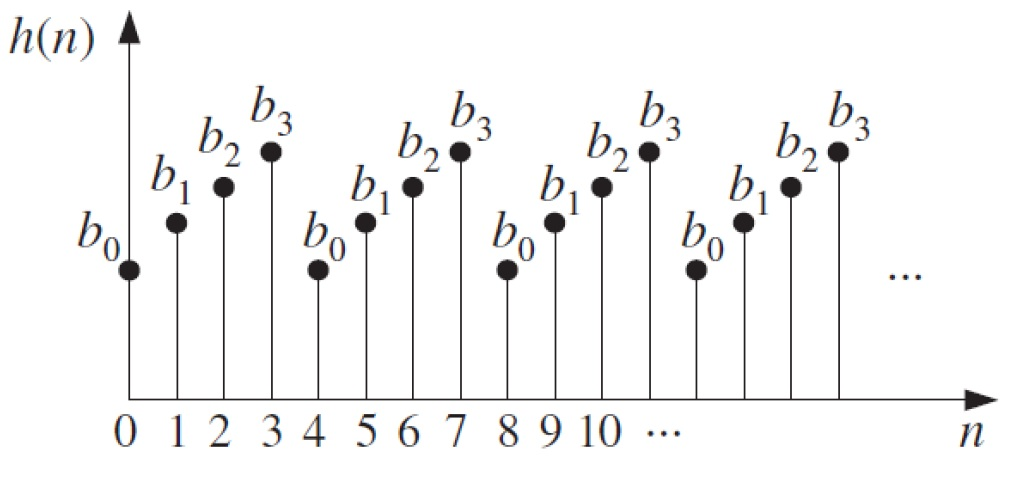
\includegraphics[width=6cm]{images/SignProcApp_DigWaveFormGenerator.jpg}
\end{center}
This waveform can be sample-by-sample computed as the impulse response of the filter $H(\z)$ or it can be pre-computed and stored in memory (wavetable).
If the waveform is periodic (often) then the fundamental frequency can be controlled by the speed the wavetable is read out.

\subsubsection{Sinusodial Generators\buchSeite{316-320}}
A causal sinusoidal is implemented by
\begin{align*}
	h(n) &= R^n \sin(\omega_0 n)u(n) \\
	H(\z) &= \frac{R \sin \omega_0 \z^{-1}}{1-2R\cos \omega_0 \z^{-1} + R^2 \z^{-2}}
\end{align*}
with $\omega_0 = 2 \pi f_0 / f_s$ being the digital frequency. \\

For $R=1$, $h(n)$ is a pure sine, for $0<R<1$, $h(n)$ is a geometrically declining sinusoidal wave. \\

A cosinusoidal signal is generated similarly with
\begin{align*}
	h(n) &= R^n \cos(\omega_0 n)u(n) \\
	H(\z) &= \frac{1 - R \cos \omega_0 \z^{-1}}{1-2R\cos \omega_0 \z^{-1} + R^2 \z^{-2}}
\end{align*}

As the poles of the transfer functions are at conjugate complex locations, both generators can be combined to the \emph{coupled form}:

\begin{center}
	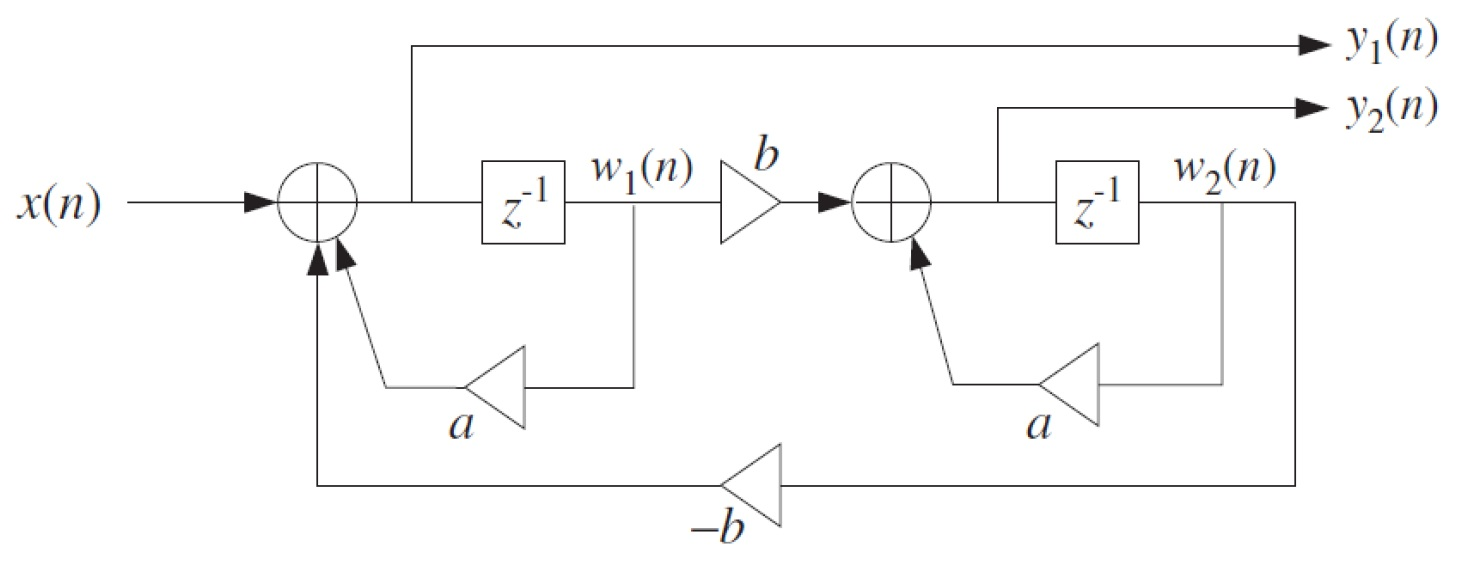
\includegraphics[width=\linewidth]{images/SignProcApp_SinCoupledForm.jpg}
\end{center}
with
\begin{equation*}
	a = R \cos \omega_0 \qquad b = R \sin \omega_0
\end{equation*}
or in the $z$-domain:
\begin{align*}
	H_1(\z) &= \frac{1 - a \z^{-1}}{1 - 2 a \z^{-1} + (a^2+b^2) \z^{-2}}  &\text{(cosine)} \\
	H_2(\z) &= \frac{b \z^{-1}}{1 - 2 a \z^{-1} + (a^2+b^2) \z^{-2}} &\text{(sine)}
\end{align*}

\subsubsection{Periodic Waveform Generators\buchSeite{321-329}}
A sampled version of a periodic signal is not necessarily periodic.
In order for $x(n)$ to be periodic in $n$ with a period of $D$ samples,
one whole period of the signal must fit within the $D$ samples.
Therefore at $n = D$ the signal must cycle by one whole period. \\

This requires that $x(D) = x(0)$, which requires
\begin{align*}
	\omega = \frac{2\pi}{D} && f = \frac{f_s}{D} && f_s = Df && T_D = DT
\end{align*}


Because of the periodicity, it is enough to specify the signal over one period only:
\begin{align*}
	h = [b_0, b_1, \ldots, b_{D-1}, \: b_0, b_1, \ldots, b_{D-1}, \: b_0, \ldots]
\end{align*}

With the corresponding z-transform:
\begin{align*}
	H(\z) = \frac{b_0 + b_1 \z^{-1} + b_2 \z^{-2} + \ldots + b_{D-1} \z^{-(D-1)}}{1 - \z^{-D}}
\end{align*}
or the impulse response
\begin{align*}
	h(0) &= b_0 \quad h(1) = b_1 \quad \ldots \quad h(D-1) = b_{D-1} \\
	h(n) &= h(n-D) \quad \text{for } n \geq D
\end{align*}

The canonical realization is the following:
\begin{center}
	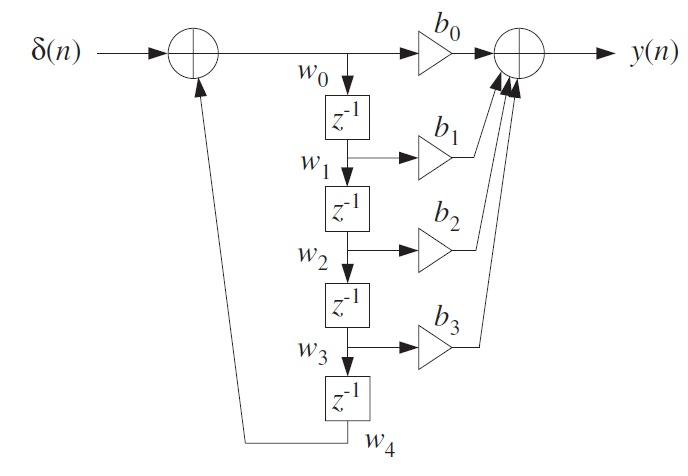
\includegraphics[width=\linewidth]{images/SignProcApp_PeriodicWaveFormGen.jpg}
\end{center}

The common delay line of the canonical form can be split up into two identical delay lines.
The first recursive filter creates a periodic impulse train as impulse response, which in turn creates a periodic waveform which consists of the finite impulse response of the FIR filter excited over and over again
\begin{center}
  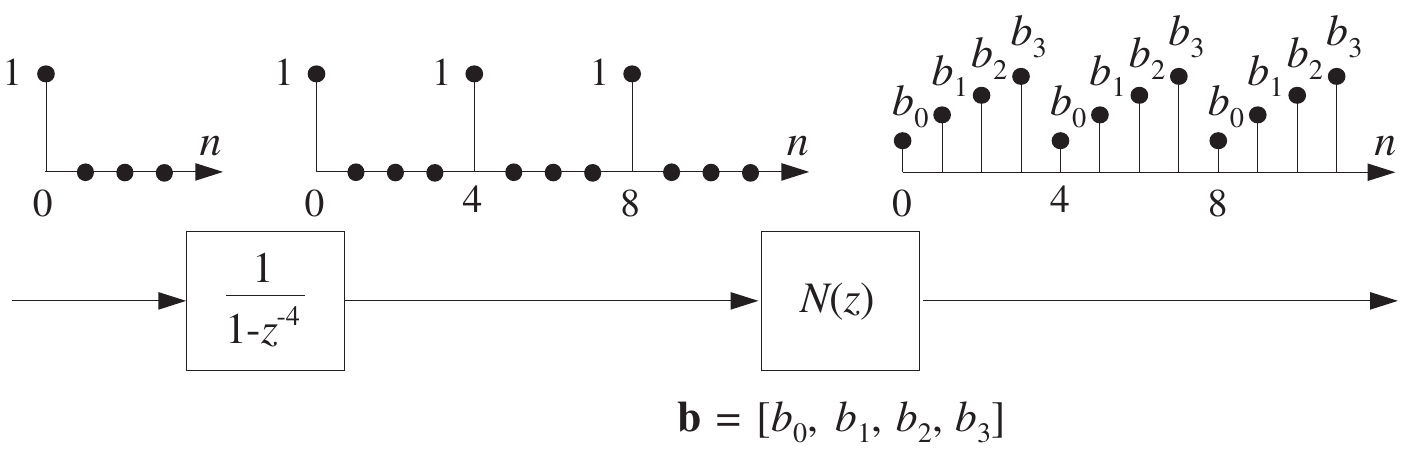
\includegraphics[width=\linewidth]{images/SignProcApp_ImpulseTrain.png}
\end{center}

These sequences are causal, therefore they have a comb-like spectra, with dominant peaks (poles) at the harmonics.
The spectrum can be obtained by setting $z=e^{jw}$ in the transfer function:
\begin{align*}
  1 - z^{-D} = ... &= 2je^{j\omega D/2}\text{sin}(\frac{\omega D}{2}) \\
  |H(\omega)| = \frac{|N(\omega)|}{|1-e^{-j\omega D}|} &= \frac{|N(\omega)|}{2|\text{sin}(\frac{\omega D}{2})|} \\
  \omega &= 2\pi f/f_s \\
  |H(f)| &= \frac{|N(f)|}{2|\underbrace{\text{sin}(\frac{\pi fD}{f_s})}_{=0}|} \\
  \Rightarrow \frac{\pi fD}{f_s} &= \pi m \\
  \Leftrightarrow f_m = m\frac{f_s}{D} = mf_1 &\quad f_1 \text{: fundamental frequency}
\end{align*}
\begin{center}
  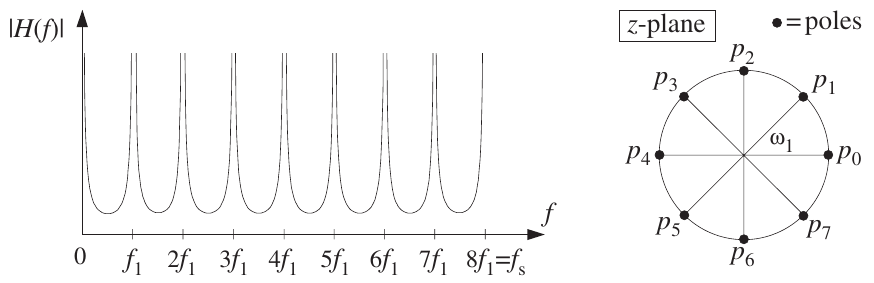
\includegraphics[width=\linewidth]{images/SignProcApp_Spectrum.png}
\end{center}


\subsubsection{Wavetable Generators\buchSeite{330-349}}
An alternative approach is to store the samples of a period in memory and
play this sample over and over again. This is called a wavetable $\mathbf{w}$. The readout is accomplished using a circular pointer $p$ and, if needed, an offset index $q$.

\begin{center}
	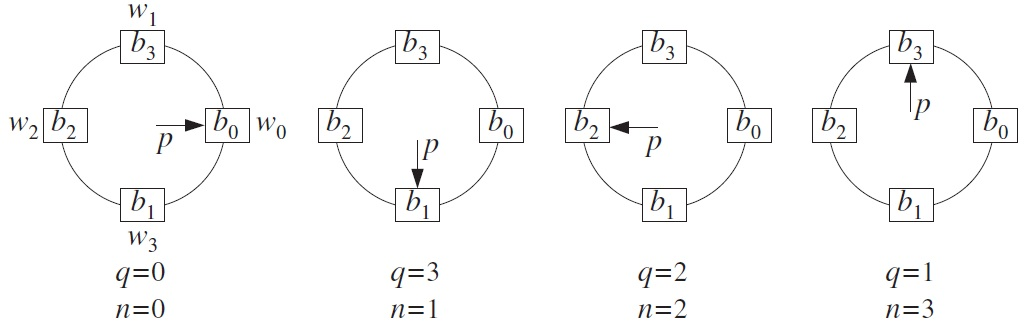
\includegraphics[width=\linewidth]{images/SignProcApp_Wavetable.jpg}
\end{center}

The wave can easily be delayed by $m$ time units by setting
\begin{equation*}
	y(n) = b(n-m)
\end{equation*}
This is achieved by initializing $p$ and $q$ with
\begin{equation*}
	p = w+m \quad q=m
\end{equation*}

This leads to the following sequences for different $m$'s

\begin{align*}
	m=0 \quad &[b_0,b_1,b_2,b_3,b_0,b_1,b_2,b_3,b_0,b_1,b_2,b_3,\ldots] \\
	m=1 \quad &[b_3,b_0,b_1,b_2,b_3,b_0,b_1,b_2,b_3,b_0,b_1,b_2,\ldots] \\
	m=2 \quad &[b_2,b_3,b_0,b_1,b_2,b_3,b_0,b_1,b_2,b_3,b_0,b_1,\ldots] \\
	m=3 \quad &[b_1,b_2,b_3,b_0,b_1,b_2,b_3,b_0,b_1,b_2,b_3,b_0,\ldots]
\end{align*}

The wavetable information can be manipulated in many possible ways to achieve
particular effects. A wavetable of length $D$ has a fundamental frequency $f$
of $f = \frac{f_s}{D}$. A shorter period $d \leq D$, meaning a higher frequency
$f = \frac{f_s}{d}$ can easily be achieved by skipping samples. \\

The constant $c = \frac{D}{d}$ describes, how often the sub-period $d$ fits into the original period $D$. To keep $f$ within the symmetric Nyquist interval, $c$ has to be inside the range

\begin{equation*}
	-\frac{D}{2} \leq c \leq \frac{D}{2}
\end{equation*}.

The update of the offset $q$ is
\begin{equation*}
	q_{n+1} = \left( q_n - c \right) \% D
\end{equation*}

Non-integer offsets can be truncated, rounded or, if higher quality is needed, interpolated.


\subsection{Noise Reduction and Signal Enhancement\buchSeite{382}}
Goal: extracting a signal from a noisy measurement. \\

\begin{tabularx}{\linewidth}{lX}
	Noisy measurement & $x(n) = s(n) + \nu(n)$ \\
	Desired signal & $s(n)$ \\
	Undesired noise & $\nu(n)$ \\
\end{tabularx} \\

\subsubsection{Noise Reduction Filters\buchSeite{382-386}}

The ideal noise reduction filter creates the output
\begin{equation*}
	y(n) = y_s(n) + y_{\nu}(n) \quad \text{with} \quad
		\begin{array}{l}
		y_s(n) = s(n) \\
		y_{\nu}(n) = 0
		\end{array}
\end{equation*}

The power spectral density of the output is calculated as
\begin{equation*}
	S_{yy}(\omega) = \left| H(\omega) \right|^2 S_{xx}(\omega)
\end{equation*}

with
\begin{equation*}
	\left| H(\omega) \right|^2 = H(\omega) \cdot H^*(\omega)
\end{equation*}

and with white noise as the input $S_{xx} = \sigma_x^2$
\begin{equation*}
	S_{yy}(\omega) = \left| H(\omega) \right|^2 \sigma_x^2
\end{equation*}

Not that the output noise is not white anymore and is therefore colored noise. \\

The \emph{noise reduction ratio} $\NRR$ measures the noise power at the output
compared to the noise power at the input. Note that a small NRR means
large noise reduction.
\begin{equation*}
	\NRR = \frac{\sigma_y^2}{\sigma_x^2}
		 = \int\limits_{-\pi}^{\pi} \left| H(\omega) \right|^2 \frac{d\omega}{2\pi}
		 = \sum\limits_{n} h(n)^2
\end{equation*}

The \emph{signal to noise ratio} $\SNR$ can be calculated at the input and
at the output, hence the relative improvement of the SNR is
\begin{equation*}
	\frac{\SNR_{\text{out}}}{\SNR_{\text{in}}} = \frac{1}{\NRR} \cdot \frac{E\left[y_s(n)^2\right]}{E\left[s(n)^2\right]}
\end{equation*}

or if the desired signal $s(n)$ is not changed by the filter
\begin{equation*}
	\frac{\SNR_{\text{out}}}{\SNR_{\text{in}}} = \frac{1}{\NRR}
\end{equation*}

The best possible $\NRR$ is achieved by using ideal filters:

\begin{tabularx}{\linewidth}{lX}
	Ideal lowpass filter & $\NRR = \frac{\omega_c}{\pi}$ \\
	Ideal bandpass filter & $\NRR = \frac{\omega_b - \omega_a}{\pi}$ \\
\end{tabularx} \\

Most real noise reduction filters are linear phase filters, where each frequency is delayed by the same number of samples and implies constant phase delay:
\begin{align*}
  y_s(n) = s(n-D)
\end{align*}

\paragraph{First-order IIR Smoother\buchSeite{386}}
To remove zero-mean white Gaussian noise of variance $\sigma_v^2$, an
IIR lowpass filter is used:
\begin{equation*}
	H(\z) = \frac{b}{1-a\z^{-1}}
\end{equation*}

With $0 < a < 1$ and $H(1)=1$, $b$ can be fixed to $b=1-a$. In that
case the $\NRR$ is
\begin{equation*}
	\NRR = \frac{b^2}{1-a^2} = \frac{1-a}{1+a}
\end{equation*}

The transient time constant will be
\begin{equation*}
	n_{\text{eff}} = \frac{\ln \epsilon}{\ln a} \to \infty \quad \text{as} \quad a \to 1
\end{equation*}
The one-percent time constant is of course
 $n_{\text{eff}}=\frac{\ln(0.01)}{\ln(a)}$ \\

The 3-DB cutoff frequency $\omega_c$ is calculated at
$\left| H(\omega_c) \right|^2 = \frac{1}{2}$, leading to
\begin{equation*}
	\omega_c = 1 - \frac{(1-a)^2}{2 a} \stackrel{\text{for } a \lesssim 1}{\backsimeq} 1-a
\end{equation*}

\paragraph{Highpass signal extraction filter\buchSeite{389}}
The $\NRR$, $n_{\text{eff}}$ and $\omega_c$ for a highpass IIR filter with
\begin{equation*}
	H(\z) = \frac{b}{1+a\z^{-1}}
\end{equation*}
can be calculated similarly, leading to the same results:
\begin{equation*}
	\NRR = \frac{1-a}{1+a} \qquad n_{\text{eff}} = \frac{\ln \epsilon}{\ln a} \qquad \omega_c \lesssim 1-a
\end{equation*}

\paragraph{First-order IIR smoother with prescribed cutoff frequency\buchSeite{390}}
By adding a zero at $\z=-1$, the $\NRR$ can be slightly improved.
The filter will be
\begin{equation*}
	H(\z) = \frac{b \left( 1 + \z^{-1} \right)}{1 - a \z^{-1}}
\end{equation*}
with $b = \frac{1-a}{2}$ for unity gain at DC. The NRR of this filter will be
\begin{equation*}
	\NRR = \frac{1-a}{2}
\end{equation*}
The following equations are used to determine $\omega_c$ or $a$.
\begin{equation*}
	\cos \omega_c = \frac{2 a}{1+a^2} \Leftrightarrow a = \frac{1-\tan(\omega_c/2)}{1+\tan(\omega_c/2)}
\end{equation*}

\paragraph{FIR averaging filters\buchSeite{391}}
For a FIR filter, the $\NRR$ will always be
\begin{equation*}
	\NRR = \sum\limits_n h_n^2
\end{equation*}
A filter minimizing the $\NRR$ is obtained by setting $h_n = \frac{1}{N}$, which is a simple averaging filter. The $\NRR$ will be
\begin{equation*}
	\NRR = \frac{1}{N}
\end{equation*}
The length $N$ of a FIR filter should be chosen like the time constant
$n_{\text{eff}}$ for an IIR filter:
$N = n_{\text{eff}} = \frac{\ln \epsilon}{\ln a}$ \\

The cutoff frequency of an FIR averaging filter is
\begin{equation*}
	\omega_c = \frac{\pi}{N}
\end{equation*}

\paragraph{Highpass FIR signal extraction\buchSeite{396}}
The lowpass filter is changed to a highpass filter by substituting $\z \to -\z$,
changing the impulse response to $h_n \to (-1)^n h_n$, leading to
a highpass FIR filter with the impulse response
\begin{equation*}
	h_n = (-1)^n \frac{1}{N}
\end{equation*}
The noise reduction ratio stays the same.

\paragraph{Bandpass signal extraction\buchSeite{397}}
A FIR bandpass filter is achieved by a resonator filter with poles at $z = R e^{\pm j \omega_0}$.
\begin{align*}
	H(\z) &= \frac{G}{1 + a_1 \z^{-1} + a_2 \z^{-2}} \\
	h_n &= \frac{G}{\sin \omega_0} R^n \sin\left(\omega_0 n + \omega_0\right) u(n)
\end{align*}
where $a_1 = -2R \cos\omega_0$ and $a_2 = R^2$. \\

The $\NRR$ of this filter will be
\begin{equation*}
	\NRR= \frac{(1-R)(1+R^2)(1-2R\cos(2\omega_0)+R^2)}{(1+R)(1-2R^2\cos(2\omega_0)+R^4)}
\end{equation*}

The recovered sinusoid will be shifted by the phase delay $d$ of
\begin{equation*}
	d(\omega_0) = - \frac{\arg H(\omega_0)}{\omega_0}
\end{equation*}


\subsubsection{Notch and Comb Filters\buchSeite{398-406}}

Two special cases of the signal enhancement/noise reduction problem arise when:
\begin{enumerate}
	\item The noise signal $\nu(n)$ is periodic. The ideal filter will then
	be a notch filter.
	\item The desired signal $s(n)$ is periodic. The ideal filter will then
	be a comb filter.
\end{enumerate}

Usually all the harmonics of the fundamental frequency $f_1$ must be canceled.
The sampling rate $f_s$ is then chosen to be a multiple $f_1$:
\begin{equation*}
	f_s = D f_1
\end{equation*}
The noise harmonics then occur at the $D^{\text{th}}$ roots-of-unit frequencies:
\begin{equation*}
	f_k = k \frac{f_s}{D}
\end{equation*}

\paragraph{Notch filters}The notch filter is then given by
\begin{equation*}
	H_{\text{notch}}(\z) = b \frac{1-\z^{-D}}{1-a\z^{-D}}
\end{equation*}
with $b = \frac{1+a}{2}$ and $a = \rho^D$. Again $a$ must be in the interval
$0 \leq a < 1$. \\

For a given $\Delta\omega$ of the notch dips, $a$ and $b$  are obtained by
\begin{equation*}
	\beta = \tan\left(\frac{D\Delta\omega}{4}\right) \qquad a = \frac{1-\beta}{1+\beta} \qquad b = \frac{1}{1+\beta}
\end{equation*}

\paragraph{Comb filters}
As a multi-notch filter can be obtained from a single notch filter using the
substitution $\z \to \z^D$, which creates $D$ replicas in the Nyquist band,
any narrow lowpass filter can be transformed into a comb filter.
\begin{equation*}
	H(\z) = b \frac{1+\z^{-1}}{1-a\z^{-1}} \quad \to \quad
	H_{\text{comb}}(\z) = b \frac{1+\z^{-D}}{1-a\z^{-D}}
\end{equation*}

Given a 3-dB width for the peaks, the parameters can be calculated by
\begin{equation*}
	\beta = \tan\left(\frac{D\Delta\omega}{4}\right) \qquad
	a = \frac{1-\beta}{1+\beta} \qquad b = \frac{\beta}{1+\beta}
\end{equation*}

Note that the presented notch and comb filters are complementary, i.e.
\begin{equation*}
	\left|H_{\text{comb}}(\omega)\right|^2 + \left|H_{\text{notch}}(\omega)\right|^2 = 1
\end{equation*}

The $\NRR$s are the same as the $\NRR$s for the simple smoothers, as the
transform $\z \to \z^{D}$ simply inserts $D-1$ zeros in the original
impulse response. Hence the sum does not change and the $\NRR$s don't change.


\subsubsection{Signal Averaging\buchSeite{421-427}}
Signal averaging is equivalent to comb filtering, but with an FIR filter
instead of an IIR one. It is derived by applying the transform $\z \to \z^{-1}$
to the FIR averaging filter of length $N$:

\begin{align*}
	H(\z)&=\frac{1}{N}\left( 1+ \z^{-D}+\z^{-2D}+\ldots + \z^{-(N-1)D} \right) \\
	&= \frac{1}{N}\frac{1-\z^{-ND}}{1-\z^{-D}}
\end{align*}

Again, the $\NRR$ stays the same: $\NRR = \frac{1}{N}$. \\

In the time domain, the filter is given by the following I/O difference equation:

\begin{equation*}
	y(n) = \frac{1}{N} \left[ x(n)+x(n-D)+\ldots+x(n-(N-1)D) \right]
\end{equation*}

As the IIR comb filter is more efficient, it is mostly used for real time
processing. The FIR averaging filter is used when measuring a finite number
$N$ of periods of the same noisy signal. \\

For $N$ periods of $D$ samples, the total length will be $ND$. The $i$th period
of the signal will then be
\begin{equation*}
	x_i(n) = x(iD+n)
\end{equation*}
where $i=0,1,\ldots,N-1$ for a total of $N$ periods. \\

The output will then be
\begin{equation*}
	\hat{y}(n)=\frac{1}{N}\sum_{i=0}^{N-1}x_i(n)
\end{equation*}

and the noise will, of course, be reduced by a factor of the $\NRR$, i.e.
\begin{equation*}
	\sigma_{\hat{v}}^2 = \frac{1}{N} \sigma_v^2
\end{equation*}


\subsubsection{Savitzky-Golay Smoothing Filters\buchSeite{427-451}}

The Savitzky-Golay smoothing filters (also: polynomial smoothing or
least-squares smoothing filters) are an elegant generalization of the
simple FIR averaging filter. \\

It optimally fits a set of data points to a polynomial of a specified
degree in least-squares sense.

\begin{center}
	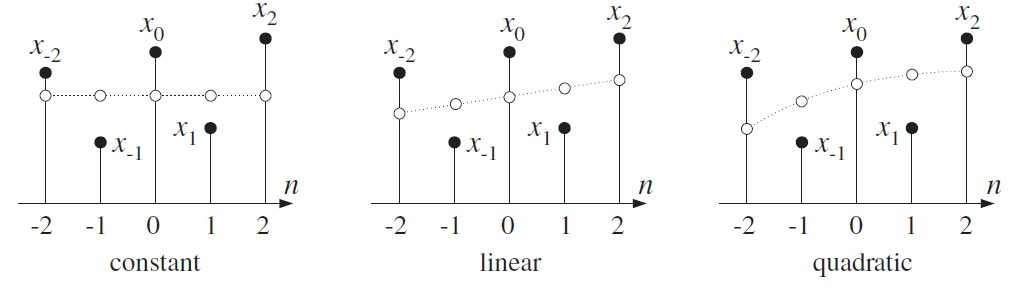
\includegraphics[width=\linewidth]{images/SignProcApp_SavitzkyGolay.jpg}
\end{center}

The smoothed value $\hat{x}_m$ at each point is given by
\begin{equation*}
	\hat{x}_m = c_0 \qquad \hat{x}_m = c_0 + c_1 m \qquad \hat{x}_m = c_0 + c_1 m + c_2 m^2
\end{equation*}
with the free variable $m = -2,-1,0,1,2$. \\

The coefficients $c_i$ now have to be
optimally found in a least-squares sense, using linear algebra. \\

We  therefore introduce \emph{basis vectors}
$\mathbf{s}_0, \mathbf{s}_1, \mathbf{s}_2$, whose components are (quadratic approx.):
\begin{equation*}
	\mathbf{s}_0(m) = 1 \qquad \mathbf{s}_1(m) = m \qquad \mathbf{s}_2(m) = m^2 \\
\end{equation*}
Therefore
\begin{equation*}
	\hat{\mathbf{x}} = \left[\mathbf{s}_0,\mathbf{s}_1,\mathbf{s}_2\right]
	\begin{bmatrix}c_0\\c_1\\c_2\end{bmatrix} = S\mathbf{c}
\end{equation*}
with the optimal coefficients
\begin{equation*}
	\mathbf{c} = G^T \mathbf{x} \qquad \text{with} \qquad G = S \left(S^T S \right)^{-1}
\end{equation*}
Inserting the optimal coefficients, we find
\begin{equation*}
	\hat{\mathbf{x}} = S G^T \mathbf{x} = B \mathbf{x} \quad \text{with} \quad B = S G^T = S \left(S^T S\right)^{-1} S^T
\end{equation*}

And therefore the output smoothed value
\begin{equation*}
	y_0 = \hat{x}_0 = c_0 = \mathbf{b}_0^T \mathbf{x} = \mathbf{g}_0^T \mathbf{x}
\end{equation*}

This can be realized as a regular FIR filter, which is in case of the 2nd order
polynomial
\begin{equation*}
	y_0 = \frac{1}{35} \left( -3 x_{n-2} + 12 x_{n-1} + 17 x_n + 12 x_{n+1} - 3 x_{n+2}\right)
\end{equation*}

The $\NRR$ of Savitzky-Golay filters is the middle coefficient:
\begin{equation*}
	\NRR = \mathbf{b}_0^T \mathbf{b}_0 = b_0(0) = \frac{17}{35} = 0.49
\end{equation*}

\paragraph{Savitzky-Golay for derivatives}
Focus on the middle value at $m=0$:
\begin{equation*}
	\hat{x}_m = c_0 + c_1 m + c_2 m^2
\end{equation*}
Clearly the derivatives are
\begin{align*}
	\dot{\hat{x}}_0 &=  \left.\frac{d\hat{x}_m}{dm}\right|_0 = c_1 = \mathbf{g}_1^T\mathbf{x} \\
	\ddot{\hat{x}}_0 &= \left.\frac{d^2\hat{x}_m}{dm^2}\right|_0 = 2 c_2 = 2 \mathbf{g}_2^T\mathbf{x}
\end{align*}
and can be written as FIR filters
\begin{align*}
	\dot{y}_n &= \frac{1}{35} \left( -7 x_{n-2} - 3.5 x_{n-1} + 3.5 x_{n+1} + 7 x_{n+2}\right) \\
	\ddot{y}_n &= \frac{2}{35} \left( 5 x_{n-2} - 2.5 x_{n-1} - 5 x_n - 2.5 x_{n+1} + 5 x_{n+2}\right)
\end{align*}

\paragraph{Savitzky-Golay for integrals}
The same concepts of course also apply to  the integral $i$:
\begin{align*}
	i_n &= \int\limits_{-1/2}^{1/2} \hat{x}_m dm = \int\limits_{-1/2}^{1/2} (c_0 + c_1 m + c_2 m^2) dm \\
	&= \left[1 \: 0 \: 1/12 \right] \cdot \mathbf{c} = \left[1 \: 0 \: 1/12 \right] \left(S^T S \right)^{-1} S^T \mathbf{x}
\end{align*}
which leads to
\begin{align*}
	\dot{y} = & \left(-0.0738 x_{n-2} + 0.3369 x_{n-1} + \right. \\
	& \left. 0.4738 x_n + 0.3369 x_{n+1} - 0.0738 x_{n+2}  \right) \\
\end{align*}

\paragraph{Generalization}
So far, the length was $N=5$ and the degree $d=2$. Of course this can easily be
generalized to any odd $N \geq d+1$.
\begin{align*}
  N &= 2M + 1 \\
  \mathbf{x} &= [x_{-M},\ldots,x_{-1},x_0,x_1,\ldots,x_M]^T \\
  \hat{x}_m &= c_0 + c_1m + \ldots + c_dm^d, \quad -M \leq m \leq M
\end{align*}


\section{DFT/FFT Algorithms\buch{Chapter 9}}
\subsection{Begriffe}

\begin{tabularx}{\textwidth}{l p{3cm}XX}
	Abkürzung & Name  & Eigenschaft & Anwendung \\\hline
	DTFT &
	discrete-time Fourier transform &
	bildet ein endliches, zeitdiskretes Signal auf ein kontinuierliches, periodisches Frequenzspektrum ab &
	Im Spektrum lässt sich unter Umständen  abschnittsweise ein geschlossener mathematischer Ausdruck angeben \\
	DFT &
	discrete Fourier transform &
	bildet ein zeitdiskretes, endliches Signal, welches periodisch fortgesetzt wird, auf ein diskretes, periodisches Frequenzspektrum ab &
	DFT besitzt zur Signalanalyse große Bedeutung \\
	FFT &
	fast Fourier transform &
	ein Algorithmus zur effizienten Berechnung der Werte einer diskreten Fourier-Transformation (DFT) &
	\vspace{-19pt}
	\begin{itemize}
		\item Zur Reduzierung des Berechnungsaufwandes bei der zirkularen Faltung
		\item im Zeitbereich von FIR-Filtern
		\item Ersatz durch die schnelle Fouriertransformation und einfache Multiplikationen im Frequenzbereich
		\item Synthese von Audiosignalen aus einzelnen Frequenzen über die inverse FFT
	\end{itemize}\\
\end{tabularx}

\subsection{Frequency Resolution and Windowing\buchSeite{464-472}}
\begin{tabular}{|l|l|l|}
	\hline
	symbol & property & formulas
	\\ \hline
	$T_L$ & duration of data record & $ = LT$
	\\ \hline
	$w(n)$ & Window function &
	\\ \hline
	$\Delta \omega_w$ & Window width (rad/sample) & $ = c \frac{2 \pi}{L}$
	\\ \hline
	$\Delta f_w$ & Window width (Hz) & $ = c \frac{f_s}{L} = c \frac{1}{T_L} $
	\\ \hline
	$\Delta f$ & Frequency resolution & $ \Delta f \geq \Delta f_w=c\frac{f_s}{L}=c\frac{1}{T_L}$
	\\ \hline
	$\Delta\omega$ & Resolvability condition & $=\Delta\omega \geq \Delta\omega_w = c\frac{2\pi}{L}$ 
	\\\hline
	$R$ & relative sidelobe level &
	\\ \hline
	$c$ & depends on window, always $\geq 1$ &
	\\ \hline
\end{tabular}


\begin{flalign*}
& \text{Window/Funktion} && \text{Rectangular} && \text{Hamming}\\
& w(n) &&  \begin{cases}
			1, & \text{if } 0 \leq n \leq L-1 \\
			0, & \text{otherwise}
 \end{cases} &&
\begin{cases}
	0.54 - 0.46 \cos(\frac{2\pi n}{L-1}), & \text{if } 0 \leq n \leq L-1 \\
	0, & \text{otherwise}
\end{cases} \\
& \text{window tradeoff } c && c=1 && c=2\\
& R && -13.46 dB && -40 dB\\
& x_{_L}(n) && x(n)w(n) && \\
& X_{_L}(\omega) && \int_{-\pi}^{\pi}X(\omega')W(\omega-\omega')\frac{d\omega'}{2\pi} && \\
\end{flalign*}



\subsection{DTFT Computation}
\subsubsection{DTFT at a Single Frequency\buchSeite{475-477}}
\begin{align*}
X(\omega)=\sum_{n=0}^{L-1}x(n)e^{-j\omega n}=\sum_{n=0}^{L-1}x(n)z^{-n}\biggr|_{z=e^{j\omega}}=X(z)\biggr|_{z=e^{j\omega}}
\end{align*}

For example let L
\begin{flalign*}
& X && = && x_3+z^{-1}X && = && x_3\\
& X && = && x_2+z^{-1}X && = && x_2+z^{-1}x^3\\
& X && = && x_1+z^{-1}X && = && x_1+z^{-1}x_2+z^{-2}x_3\\
& X && = &&  x_0+z^{-1}X && = && x_0+z^{-1}x_1+z^{-2}x_2+z^{-3}x_3 && = && X(z)&&\\
\end{flalign*}

\subsubsection{DTFT over a Frequency Range\buchSeite{478}}
\begin{align*}
\omega_k=\frac{2\pi k}{N}&& f_k=\frac{kf_s}{N} && z_k=e^{j\omega_k}=e^{2\pi jk/N} && k=0,1,\ldots , N-1 
\end{align*}
\begin{align*}
X(\omega_k)=\sum_{n=0}^{L-1}x(n)e^{-j\omega_kn} = \sum_{n=0}^{L-1}x(n)z_k^{-n} && \text{mit} && z_k=e^{j\omega_k} = z_k=e^{n\pi j k /N}
\end{align*}
\begin{align*}
\omega_k=\omega_a+k\frac{\omega_b-\omega_a}{N}=\omega_a+k\Delta\omega_{bin} && \omega_{bin}=\frac{\omega_b-\omega_a}{N} && \text{or in Hz} && \Delta f_{bin}=\frac{f_b-f_a}{N} && \omega_{k+N}=\omega_k+2\pi
\end{align*}

\subsubsection{DFT\buchSeite{479-481}}
\begin{align*}
\omega_k=\frac{2\pi k}{N}&& f_k=\frac{kf_s}{N} && z_k=e^{j\omega_k}=e^{2\pi jk/N} && k=0,1,\ldots , N-1 
\end{align*}
\begin{align*}
X(\omega_k)=\sum_{n=0}^{L-1}x(n)e^{-j\omega_kn} = \sum_{n=0}^{L-1}x(n)z_k^{-n} && \text{mit} && z_k=e^{j\omega_k} = z_k=e^{n\pi j k /N}
\end{align*}
\begin{align*}
\Delta_{bin}=\frac{2\pi}{N} && \text{or} && \Delta f_{bin}=\frac{f_s}{N} && \omega_{k+N}=\omega_k+2\pi
\end{align*}
\subsubsection{Zero Padding\buchSeite{482}}
Alle an das Signal angehängten '0' ändern die DTFT nicht 
\begin{align*}
x= [x_0,x_1,\ldots,x_{L-1}] && x_D=[x_0,x_1,\ldots,x_{L-1},\underbrace{0,0,\ldots,0}_{D zeros}] && X_D(\omega_k)=X(\omega_k)\\
\end{align*}

Alle vor das Signal angehängten '0' verschieben das Original Signal zurück
\begin{align*}
x= [x_0,x_1,\ldots,x_{L-1}] && x_D=[\underbrace{0,0,\ldots,0}_{D zeros},x_0,x_1,\ldots,x_{L-1}] \\
X_D(\omega)=e^{-j\omega D}X(\omega) && X_D(\omega_k)=e^{-j\omega_k D}X(\omega_k) && k=0,1,\ldots,N-1
\end{align*}

\subsection{Physical versus Computional Resolution\buchSeite{482-485}}
Eine künstliche Frequenzauflösung mittels Vergrösserung des N kann keine peaks die mit zu kleinem L verpasst wurden wieder rekonstruieren. 

\begin{align*}
f_0 = f_{k_0}=\frac{k_0f_s}{N} && k_0=N\frac{f_0}{k_s} && k=N\frac{f}{f_s} && 0 \leq f \leq f_s && 0 \leq k \leq N
\end{align*}

\subsection{Matrix Form of DFT\buchSeite{486-488}}
\begin{align*}
X=DFT(x)=Ax && X_k=\sum_{n=0}^{L-1}A_{kn}x_n && k=0,1,\ldots,N-1
\end{align*}
\begin{align*}
\text{2-point} && W_2=e^{-2\pi j/2}=-1 &&
 A=
\begin{bmatrix}
1 & 1  \\
1 & W_2 
\end{bmatrix}
=
\begin{bmatrix}
1 & 1  \\
1 & -1 
\end{bmatrix}\\
\text{4-point}&& W_4=e^{-2\pi j/4}=-j &&
A=
\begin{bmatrix}
1 & 1 & 1 & 1  \\
1 & W_4 & W_4^2 & W_4^3 \\
1 & W_4^2 & W_4^4 & W_4^6 \\
1 & W_4^3 & W_4^6 & W_4^9
\end{bmatrix}
=
\begin{bmatrix}
1 & 1 & 1 & 1  \\
1 & -j & -1 & j  \\
1 & -1 & 1 & -1 \\
1 & j & -1 & -j
\end{bmatrix}\\
\text{8-point} && W_8=e^{-2\pi j/8}=\frac{1-j}{\sqrt{2}} &&
 A=\begin{bmatrix}
 \ldots\\
 \ldots\\
 \ldots
 \end{bmatrix}
\end{align*}

\subsection{Module-N reduction\buchSeite{489-496}}
\begin{itemize}
	\item Opposite of zero padding
\end{itemize}
\begin{flalign*}
&\tilde{x}=x_0+x_1+\ldots+x_n &&
\end{flalign*}
\begin{flalign*}
& X=Ax=[\tilde{A},\tilde{A},\ldots,\tilde{A}]\begin{bmatrix}
x_0\\x_1\\ \ldots\\x_n
\end{bmatrix}=\tilde{A}(x_0+x_1+\ldots + x_n)=\tilde{A}\tilde{x}=\tilde{X} &&
\end{flalign*}
\begin{flalign*}
& x=[\underbrace{a_1,a_2,a_3}_{x_0},\underbrace{a_4,a_5,a_6}_{x_1},\underbrace{a_7,a_8,a_9}_{x_2},\underbrace{a_{10},a_{11} , \text{fehlende Stelle} }_{x_3}]&&\\
& \tilde{x}=x_0^T+x_1^T+x_2^T+x_3^T=
\begin{bmatrix}a_1\\a_2\\a_3\end{bmatrix}+\begin{bmatrix}a_4\\a_5\\a_6\end{bmatrix}\begin{bmatrix}a_7\\a_8\\a_9\end{bmatrix}+\begin{bmatrix}a_{10}\\a_{11}\\0\end{bmatrix}&&\\ 
& \text{fehlende Stelle mit '0' auffüllen}&&
\end{flalign*}

\subsection{Inverse DFT\buchSeite{496-499}}
\begin{flalign*}
&\tilde{x}=IDFT(X)=\tilde{A}^{-1} X && \tilde{x}=IDFT(X)=\frac{1}{N}\tilde{A}^{*} X && IDFT(X) = \frac{1}{N}\left[DFT(X^*)\right]^* \label{eq:IDFT}\\
&\tilde{x}=x && \text{nur wenn} && N \geq L\notag\\
&\tilde{x}\neq x && \text{wenn} && N < L\notag
\end{flalign*}

\subsection{Sampling of Periodic Signals and the DFT\buchSeite{499-501}}
\begin{align*}
x(n)=\frac{1}{N}\sum_{k=0}^{N-1}X(\omega_k)e^{j\omega_k n} && \text{(DFS)} \\
X(\omega_k)=\sum_{k=0}^{N-1}x(n)e^{-j\omega_k n} && \text{(DFS coefficients)}
\end{align*}
\subsection{FFT\buchSeite{504-511}}

\subsection{Fast Convolution}
\subsubsection{Circular Convolution\buchSeite{516-518}}
\begin{flalign*}
& \text{Grundlage:}&& y=h\ast x && \Leftrightarrow && Y(\omega)=H(\omega)X(\omega)&&
\end{flalign*}
\begin{align*}
& \text{mittels DTFT:} && y=IDTFT(DTFT(h)DTFT(x))&&\\
& \text{mittels DFT:} && \tilde{y}=\widetilde{h\ast x}=IDFT(DFT(h)DFT(x))&&\\
&\text{Modulo-N-reduzierte Ergebnisse}&& \tilde{y}=\widetilde{h\ast x}= \widetilde{ {\widetilde{h}} \ast  x}=\widetilde{h\ast \tilde{x}}=\widetilde{\tilde{h}\ast \tilde{x}}&&\\ 
% ToDo irgend ein problem mit der widetilde, geht auch mit anderen buchstaben die nicht hoch sind nicht z.b. a
& \text{Bedingung, zirkuläre Faltung = Lineare Faltung} && \tilde{y}=y \text{ wenn } N\geq L_y=L+M&&
\end{align*}
\subsubsection{Overlap-Add and Overlap-Save Methods\buchSeite{520-522}}



\end{multicols}
\section{FIR Digital Filter Design\buch{Chapter 10}}

\subsection{Windowing Methods}
\subsubsection{Ideal Filters}
Ideal frequency responses (Fig. \ref{fig:freqresp}) are transformed into infinite impulse responses $d(k)$ (eq: \ref{eq:impresp}), which are then made finite using a particular window.

\begin{figure}[htp]
\begin{subfigure}{0.49\textwidth}
\centering
\newcommand{\coordinates}{coordinates {
(-3.14,1) (-1.569,1) (-1.571,0)
( 1.571,0) (1.569,1) ( 3.14,1)
};}
\begin{tikzpicture}[
trim axis left,
trim axis right
]
\begin{axis}[
	every axis plot post/.append style={mark=none},
	width=0.5\textwidth, height=0.25\textwidth,
	scale only axis,
	xmin=-3.14, xmax=3.14,
	ymin=0, ymax=1.2,
	xlabel=$\omega$,
	ylabel=$D(\omega)$,
	axis x line=bottom, axis y line=middle, enlargelimits=upper,
	xtick={-3.14,-1.57,0,1.57, 3.14}, xticklabels={$-\pi$, $-\omega_c$, 0, $\omega_c$, $\pi$}
	]
	\expandafter\addplot\coordinates
\end{axis}
\end{tikzpicture}
\caption{Highpass}
\end{subfigure}
\begin{subfigure}{0.49\textwidth}
\centering
\newcommand{\coordinates}{coordinates {(-3.14,0) (-1.569,0) (-1.571,1) (1.571,1) (1.569,0) (3.14,0)};}
\begin{tikzpicture}[
trim axis left,
trim axis right
]
\begin{axis}[
	every axis plot post/.append style={mark=none},
	width=0.5\textwidth, height=0.25\textwidth,
	scale only axis,
	xmin=-3.14, xmax=3.14,
	ymin=0, ymax=1.2,
	xlabel=$\omega$,
	ylabel=$D(\omega)$,
	axis x line=bottom, axis y line=middle, enlargelimits=upper,
	xtick={-3.14,-1.57,0,1.57, 3.14}, xticklabels={$-\pi$, $-\omega_c$, 0, $\omega_c$, $\pi$}
	]
	\expandafter\addplot\coordinates
\end{axis}
\end{tikzpicture}
\caption{Lowpass}
\end{subfigure}

\begin{subfigure}{0.49\textwidth}
\centering
\newcommand{\coordinates}{coordinates {
(-3.14,1) (-2.001,1) (-1.999,0) (-1.001,0) (-0.999,1)
(0.999,1) ( 1.001,0) ( 1.999,0) ( 2.001,1) ( 3.14,1)};}
\begin{tikzpicture}[
trim axis left,
trim axis right
]
\begin{axis}[
	every axis plot post/.append style={mark=none},
	width=0.5\textwidth, height=0.25\textwidth,
	scale only axis,
	xmin=-3.14, xmax=3.14,
	ymin=0, ymax=1.2,
	xlabel=$\omega$,
	ylabel=$D(\omega)$,
	axis x line=bottom, axis y line=middle, enlargelimits=upper,
	xtick={-3.14,-2, -1,0,1,2, 3.14}, xticklabels={$-\pi$, $-\omega_b$, $-\omega_a$, 0, $\omega_a$, $\omega_b$, $\pi$}
	]
	\expandafter\addplot\coordinates
\end{axis}
\end{tikzpicture}
\caption{Bandpass}
\end{subfigure}
\begin{subfigure}{0.49\textwidth}
\centering
\newcommand{\coordinates}{coordinates {
(-3.14,0) (-2.001,0) (-1.999,1) (-1.001,1) (-0.999,0)
(0.999,0) (1.001,1) (1.999,1) (2.001,0) ( 3.14,0)};}
\begin{tikzpicture}[
trim axis left,
trim axis right
]
\begin{axis}[
	every axis plot post/.append style={mark=none},
	width=0.5\textwidth, height=0.25\textwidth,
	scale only axis,
	xmin=-3.14, xmax=3.14,
	ymin=0, ymax=1.2,
	xlabel=$\omega$,
	ylabel=$D(\omega)$,
	axis x line=bottom, axis y line=middle, enlargelimits=upper,
	xtick={-3.14,-2, -1,0,1,2, 3.14}, xticklabels={$-\pi$, $-\omega_b$, $-\omega_a$, 0, $\omega_a$, $\omega_b$, $\pi$}
	]
	\expandafter\addplot\coordinates
\end{axis}
\end{tikzpicture}
\caption{Bandstop}
\end{subfigure}

\begin{subfigure}{0.49\textwidth}
\centering
\newcommand{\coordinates}{coordinates {(-3.14,-1) (3.14,1)};}
\begin{tikzpicture}[
trim axis left,
trim axis right
]
\begin{axis}[
	every axis plot post/.append style={mark=none},
	width=0.5\textwidth, height=0.25\textwidth,
	scale only axis,
	xmin=-3.14, xmax=3.14,
	xlabel=$\omega$,
	ylabel=$D(\omega)/j$,
	axis x line=middle, axis y line=middle, enlargelimits=upper,
	xtick={-3.14,0,3.14}, xticklabels={$-\pi$,  0, $\pi$}
	]
	\expandafter\addplot\coordinates
\end{axis}
\end{tikzpicture}
\caption{Differentiator}
\end{subfigure}
\begin{subfigure}{0.49\textwidth}
\centering
\newcommand{\coordinates}{coordinates {(-3.14,1) (-0.001,1) (0.001,-1) (3.14,-1) };}
\begin{tikzpicture}[
trim axis left,
trim axis right
]
\begin{axis}[
	every axis plot post/.append style={mark=none},
	width=0.5\textwidth, height=0.25\textwidth,
	scale only axis,
	xmin=-3.14, xmax=3.14,
	xlabel=$\omega$,
	ylabel=$D(\omega)/j$,
	axis x line=middle, axis y line=middle, enlargelimits=upper,
	xtick={-3.14,0,3.14}, xticklabels={$-\pi$,  0, $\pi$}
	]
	\expandafter\addplot\coordinates
\end{axis}
\end{tikzpicture}
\caption{Hilbert transformer}
\end{subfigure}

\caption{Ideal frequency responses}
\label{fig:freqresp}
\end{figure}


\begin{equation}
d(k) = \int_{-\pi}^{\pi}D(\omega) e^{j\omega k}\frac{d\omega}{2\pi} \label{eq:impresp}
\end{equation}

\begin{align*}
&\text{lowpass filter} && d(k) = \frac{sin(\omega_ck)}{\pi k} \\
&\text{highpass filter} && d(k) = \delta(k) - \frac{sin(\omega_ck)}{\pi k} \\
&\text{bandpass filter} && d(k) = \frac{sin(\omega_bk) -sin(\omega_ak)}{\pi k} \\
&\text{bandstop filter} && d(k) = \delta(k) - \frac{sin(\omega_bk) -sin(\omega_ak)}{\pi k} \\
\end{align*}

\subsubsection{Rectangular Window}
\begin{itemize}
	\item Simplest window
	\item truncate the infinite impulse response: $-M < k < M$
	\item $\rightarrow d = [d_{-M}, ..., d_{-1}, d_0, d_1, ..., d_M]$
	\item The resulting FIR Filter must be delayed by M samples \newline
	$\rightarrow h = d = [h_0, h_{M-1}, h_M, h_{M+1}, ..., h_{2M}]$
\end{itemize}


\subsubsection{Hamming Window}


\subsubsection{Kaiser Window}
\begin{align*}
	\alpha = \left\{
		\begin{array}{l l}
			0.1102(A-8.7)& \quad \text{if } A \geq 50\\
			0.5842(A-21)^{0.4}+0.07886(A-21) & \quad \text{if }21 < A < 50\\
			0 & \quad \text{if } A \leq 21
		\end{array} \right.
\end{align*}
\subsubsection{Kaiser Window for Filter Design}


\paragraph{Regeln:}~\\
pass und stopp Band sind identisch, sind sie unterschiedlich vorgegeben muss die härtere Bedingung verwendet werden \\
\begin{align*}
\delta=min(\delta_{pass},\delta_{stop})
\end{align*}
schlussendlich wird der Filter in beiden Bändern die gleiche Überschreitung haben
\begin{align*}
A=-20log_{10}\delta && \delta=10^{-A/20}
\end{align*}
Das Stopp band hat meistens die strengeren Anforderungen
\subsubsection{Kaiser Window for Spectral Analysis}

\subsection{Frequency Sampling Method}

\subsection{Other FIR Design Methods}


%!TEX root = ../DigSig2.tex
\section{IIR Digital Filter Design\buch{Chapter 11}}
\subsection{Bilinear Transformation\buchSeite{563-565}}
Designflow:
\begin{center}
\begin{tikzpicture}[
	node distance=3cm,
	block/.style={text width=2.5cm,text centered
	}]
\node[draw, block] (dfs) {digital filter specifications};
\node[draw, block, right=of dfs] (afs) {analog filter specifications};
\node[draw, block, below=1cm of dfs] (df) {digital filter \\ $H(z)$};
\node[draw, block, below=1cm of afs] (af) {analog filter \\ $H_a(s)$};
\node[draw, block, below=0cm of afs, xshift=3cm, rounded corners] (afdm) {analog filter design method};

\draw[-stealth, thick] (dfs) -- (afs) 
	node[block, midway, above] {bilinear \\ transformation}
	node[block, midway, below] {$\Omega = g(\omega)$};
\draw[-stealth, thick] (dfs) -- (df);

\draw[-stealth, thick] (af) -- (df) 
	node[block, midway, above] {bilinear \\ transformation}
	node[block, midway, below] {$s = f(z)$};
\draw[-stealth, thick] (afs) -- (af);

\draw[-stealth, thick] (afdm) -- +(-3,0);
\end{tikzpicture}
\end{center}
Maps from z-plane to the s-plane (from the analog frequency to the digital
frequency)

\begin{tabularx}{0.8\textwidth}{|l|X|X|}
	\hline
	\textbf{Filter} & \textbf{bilinear transformation} & \textbf{frequency map}
	\\ \hline
	lowpass &
	$s = f(z) = \frac{1 - z^{-1}}{1 + z^{-1}}$ &
	$ \Omega = g(\omega) = \tan(\frac{\omega}{2})$
	\\ \hline
	highpass &
	$s = f(z) = \frac{1 + z^{-1}}{1 - z^{-1}}$ &
	$ \Omega = g(\omega) = - \cot(\frac{\omega}{2})$
	\\ \hline
	bandpass &
	$s = f(z) = \frac{1 - 2cz^{-1} +z^{-2}}{1 - z^{-2}}$ &
	$ \Omega = g(\omega) = \frac{c - \cos(\omega)}{\sin(\omega)}$
	\\ \hline
	bandstop &
	$s = f(z) = \frac{1 - z^{-2}}{1 - 2cz^{-1} + z^{-2}}$ &
	$ \Omega = g(\omega) = \frac{\sin(\omega)}{\cos(\omega) - c}$
	\\ \hline
\end{tabularx}

\subsection{First-Order LP/HP, Second-Order Peaking an Notching Filters\buchSeite{566-581}}

\paragraph{Definitions}~\\
\begin{tabular}{|l|l|l|}
	\hline
	cutoff/center frequency & $f_c$ &
	\\ \hline
	sampling rate & $f_s$ &
	\\ \hline
	bandwidth & $\Delta f$ & Peaking/Notching filter only
	\\ \hline
	digital cutoff/center frequency & $\omega_c$ & $ = \frac{2\pi f_c}{f_s}$ \qquad (usually at 3dB-point)
	\\ \hline
	drop in dB at $f_c$ & $A_c$ & $= -10\log_{10}(G_c^2) = -20\log_{10}(G_c)$ \qquad (usually 3dB)
	\\ \hline
	drop factor & $G_c$ & $=10^{-A_c/20} \qquad \longrightarrow $ If $A_c = 3$dB $\rightarrow G_c^2 = 1/2$
	\\ \hline
\end{tabular}
\vfill
\begin{tabularx}{\textwidth}{|X|l|l|l|l|l|}
	\hline
	\textbf{filter} & $H(z) = $ & $H_a(s) = $ & $\alpha = $ & $a=$ & $b=$
	\\ \hline
	low-pass	&
	$b\frac{1 + z^{-1}}{1 - a z^{-1}}$ &
	$\frac{\alpha}{s + \alpha}$	&
	$ \frac{G_c}{\sqrt{1-G_c^2}}\tan\left(\frac{\omega_c}{2}\right)
	= \tan\left(\frac{\omega_c}{2}\right)\vert_{G_c^2 = \frac{1}{2}}$&
	$\frac{1 - \alpha}{1 + \alpha}$ &
	$\frac{\alpha}{1 + \alpha} = \frac{1 - a}{2}$
	\\ \hline
	high-pass &
	$b\frac{1 - z^{-1}}{1 - a z^{-1}}$ &
	$\frac{s}{s + \alpha}$ &
	$\frac{\sqrt{1-G_c^2}}{G_c}\tan\left(\frac{\omega_c}{2}\right)
	=\tan\left(\frac{\omega_c}{2}\right)\vert_{G_c^2 = \frac{1}{2}}$&
	$\frac{1-\alpha}{1+\alpha}$&
	$\frac{1}{1+\alpha} = \frac{1 + a}{2}$
	\\ \hline
	notch &
	$b\frac{1-2\cos(\omega_0) z^{-1} + z^{-2}}{1 -2b \cos(\omega_o) z^{-1} + (2b-1)z^{-2}}$&
	$\frac{s^2 + \Omega_0^2}{s^2+\alpha s + \Omega_0^2}$&
	$\frac{\sqrt{1-G_B^2}}{G_B}(1+\Omega_0^2)\tan\left(\frac{\Delta\omega}{2}\right)$&
	--&
	$\frac{1}{1+\frac{\sqrt{1-G_B^2}}{G_B}\tan\left(\frac{\Delta\omega}{2}\right)}$
	\\ \hline
	peak &
	$(1-b)\frac{1-z^{-2}}{1-2b\cos(\omega_0)z^{-1} + (2b-1)z^{-2}}$&
	$\frac{\alpha s}{s^2 + \alpha s + \Omega_0^2}$&
	$\frac{G_B}{\sqrt{1-G_B^2}}(1+\Omega_0^2)\tan\left(\frac{\Delta\omega}{2}\right)$&
	--&
	$\frac{1}{1+\frac{G_B}{\sqrt{1-G_B^2}}\tan\left(\frac{\Delta\omega}{2}\right)}$
	\\ \hline
\end{tabularx}

\paragraph{Designflow} ~\\
\begin{enumerate}
	\item Given the cutoff frequency $\omega_c$ and the corresponding gain $A_c$ in dB, compute $G_c$.
	\item Compute the analog parameter $\alpha$
	\item Compute the digital filter coefficients $\{a,b\}$.
\end{enumerate}


\subsection{Higher Order Filters\buchSeite{592-631}}
The quantities $\{\epsilon_{pass}, \epsilon_{stop}\}$ control the depths of the passband and stopband.
They can be written in the equivalent forms:
\begin{align*}
	\epsilon_{pass} &= \sqrt{10^{A_{pass}/10} - 1} & \Longleftrightarrow &&
	A_{pass}&= 10\log_{10}(1 + \epsilon_{pass}^2) \\
	\epsilon_{stop} &= \sqrt{10^{A_{stop}/10} - 1} & \Longleftrightarrow &&
	A_{stop}&= 10\log_{10}(1 + \epsilon_{stop}^2)
\end{align*}

The specifications of the equivalent analog filter are $\{\Omega_{pass}, \Omega_{stop}, A_{pass}, A_{stop} \}$, or, $\{\Omega_{pass}, \Omega_{stop}, \epsilon_{pass}, \epsilon_{stop} \}$, where the analog frequencies are obtained by pre-warping the digital frequencies.
\begin{align*}
	\Omega_{pass} &= \tan\left(\frac{\omega_{pass}}{2}\right) &
	\Omega_{stop} &= \tan\left(\frac{\omega_{stop}}{2}\right) \\
	\omega_{pass} &= \frac{2\pi f_{pass}}{f_s} &
	\omega_{stop} &= \frac{2\pi f_{stop}}{f_s}
\end{align*}

\subsubsection{Analog Lowpass Butterworth Filters\buchSeite{594-599}}
Analog lowpass Butterworth filters are characterized by just two parameters:
filter order $N$ and the 3-dB normalization frequency $\Omega_0$.
\[
	\left|H(\Omega)\right|^2 =
		\frac{1}{1 + \left(\frac{\Omega}{\Omega_0}\right)^{2N}}
\]

With the given information, we can calculate the two parameters:
\begin{align*}
	N_{exact} &= \frac{
			\ln(\epsilon_{stop} / \epsilon_{pass})
		}{
			\ln(\Omega_{stop} / \Omega_{pass})
		}
	= \frac{\ln(e)}{\ln(w)} &
	e &= \frac{\epsilon_{stop}}{\epsilon_{pass}}
	   = \sqrt{\frac{10^{A_{stop}/10} -1}{10^{A_{pass}/10} -1}}&
	w &= \frac{\Omega_{stop}}{\Omega_{pass}}&
\end{align*}

$N$ must be an integer, we round $N_{exact}$ up to the nearest integer: $N = \lceil N_{exact} \rceil$

\[
	\Omega_0 = \frac{
			\Omega_{pass}
		}{
			\left(10^{A_{pass}/10}-1\right)^{1/2N}
		} = \frac{
			\Omega_{pass}
		}{
			\epsilon_{pass}^{1/N}
		}
\]

Of course , $\Omega_0$ can be calculated in terms of the stopband. Then the
passband attenuation will be a bit smaller than necessary.

\paragraph{Spectral factorization}
The amplitude response $\left|H(\Omega)\right|^2$ now has to be transformed
into a transfer function $H(\Omega)$. With $s = j \Omega$, the fact that
$\left|H(\Omega)\right|^2 = H(\Omega) H(\Omega)^*$ and setting
$H(s) = \frac{1}{D(s)}$, we have
\begin{equation*}
	D(s) D(-s)^* = 1 + (-1)^N \left( \frac{s}{\Omega_0} \right)^{2N}
\end{equation*}

\vspace{1em}

\begin{multicols}{2}
	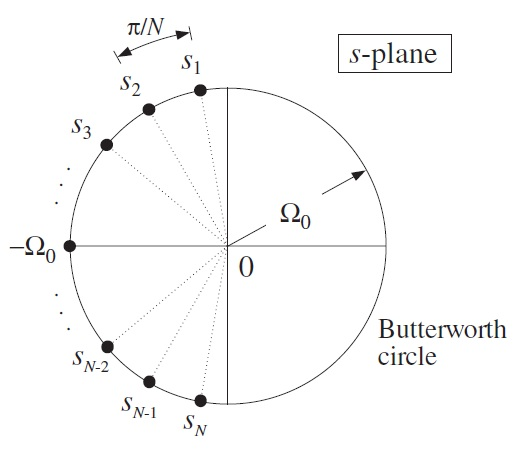
\includegraphics[width=7cm]{images/IIR_ButterworthCircle.jpg}
\vfill
\columnbreak

	To find an $H(s)$ that is causal and stable, we have to find all the roots
	in the left hand side of the s-plane of the following polynomial:
	\begin{equation*}
		1 + (-1)^N \left(\frac{s}{\Omega_0}\right)^{2N} = 0 \qquad \Rightarrow \qquad s^{2N} = (-1)^{N-1} \Omega_0^{2N}
	\end{equation*}

	The $2N$ roots are equally spaced on a circle in the s-plane with the radius
	of $\Omega_0$.
	\begin{equation*}
		s_i = \Omega_0 e^{j \theta_i} \:, \quad \theta_i = \frac{\pi}{2N} (N - 1 + 2i) \:, \quad  i = 1,2,\ldots,2N
	\end{equation*}
\end{multicols}

If $N$ is even $(N = 2K)$, there are exactly $K$ conjugate complex root pairs.
If $N$ is odd $(N = 2K+1)$, there are $k$ conjugate complex root pairs and one
single root at $s = -\Omega_0$. The conjugate complex pairs can be written as
second order section, allowing to write $H(s)$ as \\

\begin{align*}
	H(s) &= H_0(s) H_1(s) H_2(s) \ldots H_K(s) \qquad \text{where} \qquad
	\begin{array}{ll}
		H_0(s) & = \begin{cases}
			1\:, & \text{if} \quad N = 2K \\
			\frac{1}{1 + \frac{s}{\Omega_0}} \:, & \text{if} \quad N = 2K+1
			\end{cases} \\
		H_i(s) &= \frac{1}{1 - 2 \frac{s}{\Omega_0} \cos\theta_i + \frac{s^2}{\Omega_0^2}} \:,\quad i=1,2,\ldots,K
	\end{array}
\end{align*}

A list of Butterworth polynomials can be found in appendix \ref{app:Butterworth}.

\paragraph{Design steps}
\begin{enumerate}
	\item Calculate the digital frequencies $\{\omega_{pass}, \omega_{stop}\}$
	and the corresponding prewarped version $\{\Omega_{pass}, \Omega_{stop}\}$.
	\item Calculate the order $N$ and the 3-dB frequency $\Omega_0$ of the
	 equivalent analog Butterworth filter based on the transformed specifications
	 $\{\Omega_{pass}, \Omega_{stop}, A_{pass}, A_{stop} \}$
	\item Calculate the coefficients for all second-order sections and the transfer function.
\end{enumerate}

\subsubsection{Digital Lowpass Filters\buchSeite{599}}
As before, the analog lowpass filter must be transformed into a digital
filter using the bilinear transform

\begin{equation*}
	H_i(z) = \left.\frac{1}{1 - 2 \frac{s}{\Omega_0}\cos\theta_i + \frac{s^2}{\Omega_0^2}}\right|_{s = \frac{1-z^{-1}}{1+z^{-1}}} =
	\frac{G_i (1+z^{-1})^2}{1 + a_{i1}z^{-1} + a_{i2}z^{-2}}
\end{equation*}

where the filter coefficients $G_i, a_{i1}, a_{i2}$ are easily found to be

\begin{equation*}
	G_i = \frac{\Omega_0^2}{1 - 2 \Omega_0 \cos\theta_i + \Omega_0^2} \qquad
	a_{i1} = \frac{2(\Omega_0^2 - 1)}{1 - 2 \Omega_0 \cos\theta_i + \Omega_0^2} \qquad
	a_{i2} = \frac{1 + 2 \Omega_0 \cos\theta_i + \Omega_0^2}{1 - 2 \Omega_0 \cos\theta_i + \Omega_0^2}
\end{equation*}

If $N$ is odd, there is of course a first-order section

\begin{equation*}
	H_0(z) = \left.\frac{1}{1+\frac{s}{\Omega_0}}\right|_{s = \frac{1-z^{-1}}{1+z^{-1}}}
	= \frac{G_0 (1+z^{-1})}{1 + a_{01} z^{-1}}
	\qquad \text{with} \qquad
	G_0 = \frac{\Omega_0}{\Omega_0 + 1} \:,\quad
	a_{01}=\frac{\Omega_0 - 1}{\Omega_0 + 1}
\end{equation*}

This results in the overall digital transfer function
$H(z) = H_0(z) H_1(z) H_2(z) \ldots H_K(z)$. The 3dB frequency
$f_0$ in Hz is related to the Butterworth parameter $\Omega_0$ over the
bilinear transform:
\begin{equation*}
	f_0 = \frac{f_s}{\pi} \arctan(\Omega_0)
\end{equation*}

\subsubsection{Digital Highpass Filters\buchSeite{603}}
The highpass version of the bilinear transform is used to map the given
highpass specifications onto equivalent analog lowpass specifications. \\

For a highpass filter, the passband and stopband frequencies are calculated
by

\begin{align*}
	\Omega_{pass} &= \cot \left( \frac{\omega_{pass}}{2} \right)
	= \cot\left( \frac{\pi f_{pass}}{f_s} \right) \\
	\Omega_{pass} &= \cot\left(\frac{\omega_{stop}}{2}\right)
	= \cot\left(\frac{\pi f_{stop}}{f_s}\right)
\end{align*}

The highpass bilinear transform is then used to find $H(z)$
\begin{align*}
	H_i(z) &= \frac{G_i (1-z^{-1})^2}{1 + a_{i1} z^{-1}+a_{i2}z^{-2}} \\
	\text{where} \\
	G_i = \frac{\Omega_0^2}{1-2\Omega_0\cos\theta_i + \Omega_0^2} \qquad
	a_{i1} &= -\frac{2(\Omega_0^2-1)}{1-2\Omega_0\cos\theta_i + \Omega_0^2} \qquad
	a_{i2} = \frac{1 + 2\Omega_0\cos\theta_i + \Omega_0^2}{1-2\Omega_0\cos\theta_i + \Omega_0^2}
\end{align*}

Again, if $N$ is odd, then there is a first-order section
\begin{equation*}
	H_0(z) = \frac{G_0(1-z^{-1})}{1 + a_{01} z^{-1}} \qquad \text{where} \quad
	G_0 = \frac{\Omega_0}{\Omega_0 + 1} \:,\quad
	a_{01} = -\frac{\Omega_0 - 1}{\Omega_0 + 1}
\end{equation*}

The 3dB frequency $f_0$ of the highpass filter can then be calculated as
\begin{equation*}
	f_0 = \frac{f_s}{\pi} \arctan\left(\frac{1}{\Omega_0}\right)
\end{equation*}

Note the similarities and differences between the highpass and the lowpass
case: The coefficients $G_i$ and $a_{i2}$ are the same, but $a_{i1}$ has
reverse sign. The numerator of the second order sections is now $(1-z^{-1})^2$
instead of $(1+z^{-1})^2$, resulting in a zero at $z=1$ or $\omega=0$.

\subsubsection{Digital Bandpass Filters\buchSeite{606}}
The bandpass filter design works similarly. This design will result in the
same attenuation in both stopbands. Hence one must focus on the stopband
with the more stringent specification. \\

The bandpass specifications are mapped onto the entire passband
$[-\Omega_{pass}\:,\:\Omega_{pass}]$ of the analog filter by

\begin{equation*}
		\Omega = \frac{c - \cos\omega}{\sin\omega} \qquad \text{where} \qquad
		c = \frac{\sin\left(\omega_{pa}+\omega_{pb}\right)}
		{\sin\omega_{pa}+\sin\omega_{pb}}
\end{equation*}

Note that $c=\cos\omega_c$ where $\omega_c$ can be thought of as the center
frequency of the bandpass filter. In general $\omega_c$ is \emph{not} exactly
the center of the passband! \\

This results in
\begin{equation*}
	\Omega_{pass} = \left| \frac{c - \cos\omega_{pb}}{\sin\omega_{pb}} \right|
	\qquad \text{and} \qquad
	\Omega_{stop} = \min\left( |\Omega_{sa}|\:,\:|\Omega_{sb}| \right)
	\quad \text{with} \quad
	\Omega_{sa} = \frac{c-\cos\omega_{sa}}{\sin\omega_{sa}}\:, \quad
	\Omega_{sb} = \frac{c-\cos\omega_{sb}}{\sin\omega_{sb}}
\end{equation*}

Again, $H_i(z)$ and, if $N$ is odd also $H_0(z)$ are calculated as
\begin{align*}
	H_i(z) &= \frac{G_i (1-z^{-2})^2}{1 + a_{i1}z^{-1} + a_{i2}z^{-2} + a_{i3}z^{-3} + a{i4}z^{-4}}
	\qquad \text{where} \quad
	G_i = \frac{\Omega_0^2}{1-2\Omega_0\cos\theta_i+\Omega_0^2} \\
	a_{i1} &= \frac{4c(\Omega_0\cos\theta_i-1)}{1-2\Omega_0\cos\theta_i+\Omega_0^2} \qquad
	a_{i2} = \frac{2(2c^2+1-\Omega_0^2)}{1-2\Omega_0\cos\theta_i+\Omega_0^2} \\
	a_{i3} &= -\frac{4c(\Omega_0\cos\theta_i+1)}{1-2\Omega_0\cos\theta_i+\Omega_0^2} \qquad
	a_{i4} = \frac{1+2\Omega_0\cos\theta_i+\Omega_0^2}{1-2\Omega_0\cos\theta_i+\Omega_0^2} \\
	\text{and} \\
	H_0(z) &= \frac{G_0(1-z^{-2})}{1+a_{01}z^{-1}+a_{02}z^{-2}} \qquad \text{where} \\
	G_0 &= \frac{\Omega_0}{1+\Omega_0} \:,\qquad
	a_{01} = -\frac{2c}{1+\Omega_0} \:,\qquad
	a_{02} = \frac{1-\Omega_0}{1+\Omega_0}
\end{align*}

Each filter section has zeros at $z=\pm 1$, i.e. $\omega=0$ and $\omega=\pi$.
The left and the right 3dB frequencies $\omega_{0a}$ and $\omega_{0b}$ can be
calculated by
\begin{equation*}
	\tan\left(\frac{\omega_{0a}}{2}\right) = \frac{\sqrt{\Omega_0^2+1-c^2}-\Omega_0}{1+c}
	\qquad \text{and} \qquad
	\tan\left(\frac{\omega_{0b}}{2}\right) = \frac{\sqrt{\Omega_0^2+1-c^2}+\Omega_0}{1+c}
\end{equation*}

\subsubsection{Digital Bandstop Filters\buchSeite{611}}
The design of digital bandstop filters is similar to that of digital
bandpass filters.

\begin{align*}
	c &= \frac{\sin(\omega_{pa}+\omega_{pb})}{\sin\omega_{pa}+\sin\omega_{pb}}
	\:,\qquad
	\Omega_{pass} = \left| \frac{\sin\omega_{pb}}{\cos\omega_{pb}-c} \right| \\
	\Omega_{stop} &= \min\left(|\Omega_{sa}|,|\Omega_{sb}|\right)
	\qquad \text{where} \quad
	\Omega_{sa} = \frac{\sin\omega_{sa}}{\cos\omega_{sa}-c}\:,\quad
	\Omega_{sb} = \frac{\sin\omega_{sb}}{\cos\omega_{sb}-c}
\end{align*}

The bilinear transform of the second order sections is then
\begin{align*}
	H_i(z) &= \frac{G_i(1-2cz^{-1}+z^{-2})^2}{1+a_{i1}z^{-1}+a_{i2}z^{-2}+a_{i3}z^{-3}+a_{i4}z^{-4}}
	\qquad \text{where} \quad
	G_i = \frac{\Omega_0^2}{1-2\Omega_0\cos\theta_i+\Omega_0^2} \\
	a_{i1} &= \frac{4c\Omega_0(\cos\theta_i-\Omega_0)}{1-2\Omega_0\cos\theta_i+\Omega_0^2} \qquad
	a_{i2} = \frac{2(2c^2\Omega_0^2+\Omega_0^2-1)}{1-2\Omega_0\cos\theta_i+\Omega_0^2} \\
	a_{i3} &= \frac{4c\Omega_0(\cos\theta_i+\Omega_0)}{1-2\Omega_0\cos\theta_i+\Omega_0^2} \qquad
	a_{i4} = \frac{1+2\Omega_0\cos\theta_i+\Omega_0^2}{1-2\Omega_0\cos\theta_i+\Omega_0^2} \\
	\text{and} \\
	H_0(z) &= \frac{G_0(1-2cz^{-1}+z^{-2})}{1+a_{01}z^{-1}+a_{02}z^{-2}} \qquad \text{where} \\
	G_0 &= \frac{\Omega_0}{1+\Omega_0}\:,\qquad
	a_{01} = -\frac{2c\Omega_0}{1+\Omega_0} \:,\qquad
	a_{02} = -\frac{1-\Omega_0}{1+\Omega_0}
\end{align*}

Each second order section has zeros at $\omega = \pm \omega_c$,  which makes
sense for a bandstop filter. The 3dB frequencies are now
\begin{equation*}
	\tan\left(\frac{\omega_{0a}}{2}\right) = \frac{\sqrt{1+\Omega_0^2(1-c^2)}-1}{\Omega_0(1+c)}
  \qquad \text{and} \qquad
	\tan\left(\frac{\omega_{0b}}{2}\right) = \frac{\sqrt{1+\Omega_0^2(1-c^2)}+1}{\Omega_0(1+c)}
\end{equation*}

%!TEX root = ../DigSig2.tex
\section{Interpolation, Decimation and Oversampling\buch{Chapter 12}}
\subsection{Interpolation and Oversampling\buchSeite{632-637}}
Oversampling is increasing the sample rate and requires some form of interpolation. New samples at a higher sampling rate are created. These are calculated using a FIR filter. The spectrum of the low-rate and the high-rate signal are identical, if the frequency axis is not normalized.

\subsection{Interpolation Filter Design\buchSeite{638-657}}
\subsubsection{Direct form\buchSeite{638}}

\begin{center}
	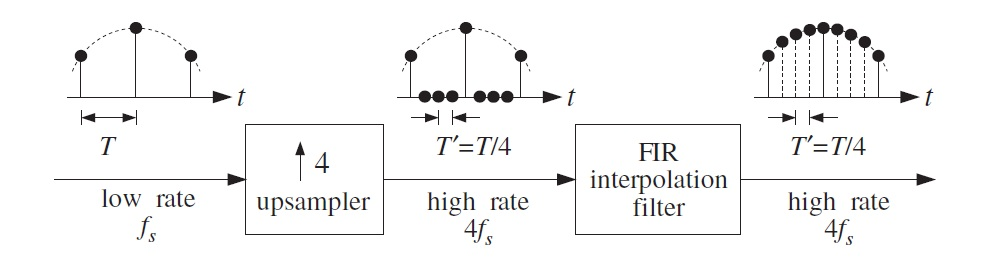
\includegraphics[width=10cm]{images/IntDecOv_IncSamplingRate.jpg}
\end{center}

There are now two discrete times, a fast one $n'$ and a slow one called $n$.
The effect on the spectrum of a signal and the advantage in DA-Conversion is
shown in the following figure (left: original spectrum, right: spectrum
at high rate).

\begin{center}
	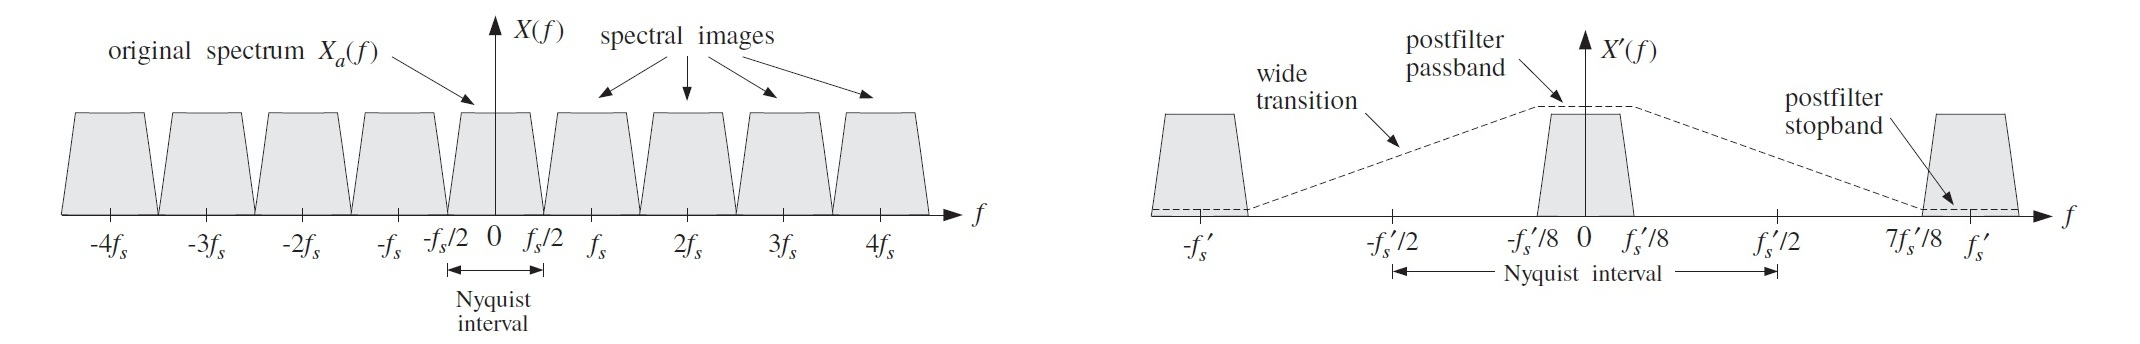
\includegraphics[width=16cm]{images/IntDecOv_Spectrum.jpg}
\end{center}

The Job of the FIR filter is to move the zeros to the appropriate values,
or to erase the spectral copies of the original spectrum in the new
Nyquist band. \\

\begin{center}
	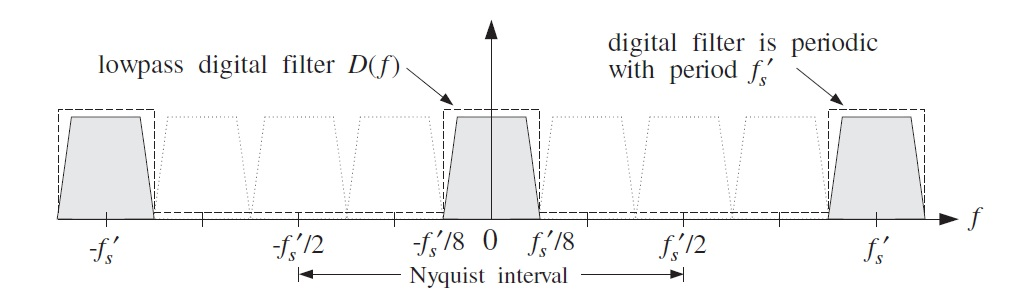
\includegraphics[width=8cm]{images/IntDecOv_Filter.jpg}
\end{center}

The ideal lowpass filter for an $L$-fold interpolation is operating at the fast
sampling rate $f'_s=L f_s$ and has its cutoff frequency at the low-sampling
rate's Nyquist frequency $f_s/2$.

\begin{equation*}
	f_c = \frac{f_s}{2}=\frac{f'_s}{2L}
	\qquad
	\omega'_c = \frac{2\pi f_c}{f'_s}=\frac{\pi}{L}
\end{equation*}

\begin{tabularx}{\linewidth}{Xl}
	FIR approximation to the ideal interpolator (non causal):
	& $d(k')=\frac{\sin(\pi k'/L)}{\pi k'/L}$, with $-LM\leq k'\leq LM$\\
	By delaying this filter by $LM$ samples, it gets causal:
	& $h(n')=d(n'-LM)=\frac{\sin(\pi (n'-LM)/L)}{\pi (n'-LM)/L}$ \\
	Using a Hamming window: & $h(n')=w(n')d(n'-LM)$ \\
	Hamming window & $w(n') = 0.54-0.46\cos(\frac{2\pi n'}{N-1})$ \\
\end{tabularx} \\

The output of the non causal FIR interpolator filter is obtained as the
convolution of the upsampled signal with the filter

\begin{equation*}
	y_{up}(n') = \sum\limits_{k'=-LM}^{LM}d(k')x_{up}(n'-k')
\end{equation*}


\subsubsection{Polyphase Form\buchSeite{640}}

\begin{multicols}{2}
	The direct form is
	\begin{center}
		\adjustbox{max width=0.7\linewidth}{\begin{tikzpicture}
[	
	sq/.style={rectangle,draw,line width=1,minimum height=1cm,minimum width=1cm}
]

\node[sq] (t1) at (1,0) {$\zeta^{-1}$};
\node[sq] (t2) at (3,0) {$\zeta^{-1}$};
\node[sq] (t3) at (5,0) {$\zeta^{-1}$};

\node[sq] (c1) at (0,-2) {$C_0$};
\node[sq] (c2) at (2,-2) {$C_1$};
\node[sq] (c3) at (4,-2) {$C_2$};
\node[sq] (c4) at (6,-2) {$C_3$};

\node[rectangle,draw,line width=1,minimum height=1cm, minimum width=8cm] (sum) at (3,-4) {$\sum$};
\node[sq] (ds) at (-1,0) {$\uparrow 4$};

\draw[thick,->]	(ds)	-- 	(t1);
\draw[thick,->]	(t1)		-- 	(t2);
\draw[thick,->]	(t2) 		-- 	(t3);

\draw[thick,->] (ds)	-|	(c1);
\draw[thick,->] (t1)		-|	(c2);
\draw[thick,->] (t2)		-|	(c3);
\draw[thick,->] (t3)		-|	(c4);

\draw[thick,->] (c1) 		-- 	(0,-3.5);
\draw[thick,->] (c2) 		-- 	(2,-3.5);
\draw[thick,->] (c3) 		-- 	(4,-3.5);
\draw[thick,->] (c4) 		-- 	(6,-3.5);

\draw[thick,->] (-2,0) -- (ds);
\draw[thick,->] (sum) -- (8,-4);


\end{tikzpicture}}
	\end{center}
\vfill\columnbreak
	A more efficient way is using the polyphase form
	\begin{center}
		\adjustbox{max width=\linewidth}{\begin{tikzpicture}
[	
	sq/.style={rectangle,draw,line width=1,minimum height=1cm,minimum width=1cm},
	rd/.style={circle,draw,line width=1,radius=0.5cm}
]

\node[sq] (t1) at (3.5,0) {$z^{-1}$};

\node[sq] (c1) at (0,-2) {$C_0$};
\node[sq] (c2) at (2,-2) {$C_1$};
\node[sq] (c3) at (5,-2) {$C_2$};
\node[sq] (c4) at (7,-2) {$C_3$};

\node (start) at (-1,0) {};

\draw[thick,->] (start) -| (c1);
\draw[thick,->] (start) -| (c2);
\draw[thick,->] (start) -- (t1);
\draw[thick,->] (t1) -| (c3);
\draw[thick,->] (t1) -| (c4);

\node[rd] (s1) at (5,-3.5) {};
\node[rd] (s2) at (7,-5) {};

\draw[thick,->] (c1) |- (s1);
\draw[thick,->] (c3) -- (s1);
\draw[thick,->] (c2) |- (s2);
\draw[thick,->] (c4) -- (s2);

\node[sq] (us1) at (8.5,-3.5) {$\uparrow 4$};
\node[sq] (us2) at (8.5,-5) {$\uparrow 4$};

\draw[thick,->] (s1) -- (us1);
\draw[thick,->] (s2) -- (us2);

\node[sq] (t2) at (10.5,-5) {$\zeta^{-1}$};
\draw[thick,->] (us2) -- (t2);

\node[rd] (s3) at (12,-4.25) {};
\node (p1) at (11,-3.5) {};

\draw[thick] (us1) -- (p1.center);
\draw[thick,->] (p1.center) -- (s3);
\draw[thick,->] (t2.east) -- (s3);

\node (end) at (13,-4.25) {};
\draw[thick,->] (s3) -- (end);

\end{tikzpicture}}
	\end{center}
\end{multicols}

Note that the direct form does all multiplications at the high rate, while
the polyphase form allows doing the multiplications at the low rate, which
makes the system more efficient. \\

Suppose the low-rate time instants are $n$, then the fast-rate time instants
can be described as $n' = NL+i$ for $i=0,1,\ldots,L-1$. The output is therefore

\begin{equation*}
	y_{up}(nL+i) = \sum\limits_{k=-M}^{M-1}\sum\limits_{j=0}^{L-1} d(kL+j) x_{up}(nL+i-kL-j)
\end{equation*}

which allows us to split the output $y_{up}$ into $y_i(n)=y_{up}(nL+i)$.
We can also define the \emph{$i$th polyphase subfilter} as

\begin{equation*}
	d_i(k) = d(kL+i) \:,\qquad -M \leq k \leq M-1 \:,\quad i=0,1,\ldots,L
\end{equation*}

The $i$th outputs can now be calculated in terms of the slow-rate samples

\begin{equation*}
	y_i(n) = \sum\limits_{k=-M}^{M-1}d_i(k) x(n-k) \:,\qquad i=0,1,\ldots,L-1
\end{equation*}

The output $y_{up}$ is now only calculated in terms of the slow sampling rate,
which decreases the computational rate in terms of multiplications per second by
a factor of $L$, from $R = NLf_s$ (direct from) to $R = Nf_s$ (polyphase form).


\subsubsection{Frequency domain characteristics\buchSeite{645}}
To discuss the interpolation in the frequency domain, we introduce the different
unit delays $z$ (low sampling rate = long delay) and $\zeta$
(high sampling rate = short delay)

\begin{equation*}
	z = \zeta^L \qquad \Leftrightarrow \qquad \zeta = z^{1/L}
\end{equation*}

The high-rate output can now be written in the $z$-Domain as

\begin{equation*}
	Y_{up}(\zeta) = \sum\limits_{i=0}^{L-1} \zeta^{-i} Y_i(\zeta^L)
	= \sum\limits_{i=0}^{L-1} z^{-i/L} Y_i(z)
\end{equation*}

which is what we already know from the time domain. The filter $D(\zeta)$
similarly is

\begin{equation*}
	D(\zeta) = \sum\limits_{i=0}^{L-1} \zeta^{-i} D_i(\zeta^L)
	= \sum\limits_{i=0}^{L-1} z^{-i/L} D_i(z)
\end{equation*}

The 0th polyphase subfilter $d_0(k)$ should of course return the same value as
the input $x(n)$, so the impulse response must be a dirac:
$d_0(k) = d(kL) = \delta(k)$. \\

The ideal filter which removes all spectral copies would generally have
the following characteristics
\begin{equation*}
	D(f) = \begin{cases}
		L\:,	& \text{if} \quad |f|\leq\frac{f_s}{2} \\
		0\:,	& \text{if} \quad \frac{f_s}{2}\leq |f|\leq\frac{f'_s}{2}
	\end{cases}
\end{equation*}

The ideal reconstructor $d(k)$, running at the higher rate $f_s'$ would
therefore be
\begin{equation*}
	d(k') = \frac{\sin(\pi k' / L)}{\pi k' / L}
\end{equation*}

This reconstructor is usually implemented using a Kaiser window design.

\subsection{Linear and Hold Interpolators\buchSeite{657-661}}
The reconstructor described above is the ideal interpolator. Nevertheless
there exist simpler interpolators, such as the linear and the hold interpolators.
Not surprising, these are not as good as the ideal interpolator, but especially
at high sample rates, the advantage of less calculations overweights the
downsides.

\subsubsection{Hold Interpolator}
\begin{multicols}{2}
	\begin{align*}
		d(k') &= \begin{cases}
			1\:, & \text{if} \quad 0\leq k' \leq L -1\\
			0\:, & \text{otherwise}
		\end{cases} \\
		y_{up}(nL+i) &= x(n) \\
		D(f) &= \frac{\sin(\pi f/f_s)}{\sin(\pi f/Lf_s)}e^{-j\pi(L-1)f/(Lf_s)}
	\end{align*}

	The polyphase subfilters $d_i(k)$ will then be

	\begin{equation*}
		d_i(k) = \delta(k)
	\end{equation*}

\vfill
\columnbreak
	\begin{center}
		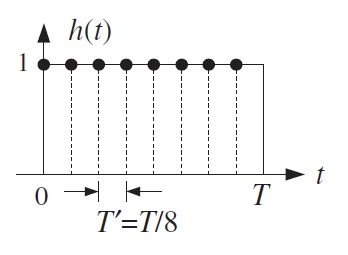
\includegraphics[width=5cm]{images/IntDecOv_Hold.jpg}
	\end{center}
\vfill
\end{multicols}

\subsubsection{Linear Interpolator}
\begin{multicols}{2}
	\begin{align*}
		d(k') &= \begin{cases}
			1-\frac{|k'|}{L}\:, & \text{if} \quad |k'|\leq L -1\\
			0\:, & \text{otherwise}
		\end{cases} \\
		y_{up}(nL+i) &= (1-\frac{i}{L})x(n)+\frac{i}{L}x(n+1) \\
		D(f) &= \frac{1}{L}\left|\frac{\sin(\pi f/f_s)}{\sin(\pi f/Lf_s)}\right|^2
	\end{align*}

	The polyphase subfilters $d_i(k)$ will then be

	\begin{equation*}
		d_i(k) = (1-\frac{i}{L}) \delta(k) + \frac{i}{L} \delta(k+1)
	\end{equation*}
\vfill
\columnbreak
	\begin{center}
		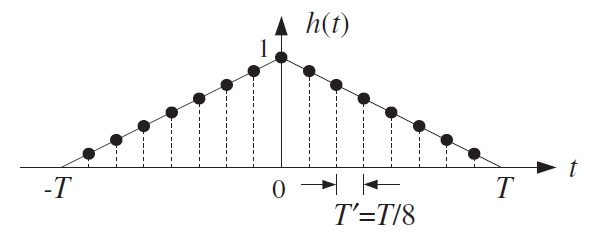
\includegraphics[width=0.8\linewidth]{images/IntDecOv_Linear.jpg}
	\end{center}
\vfill
\end{multicols}


\subsection{Design Examples\buchSeite{661-686}}
%TODO!!!!
\subsubsection{4-fold interpolators\buchSeite{661}}
\begin{equation*}
  L = 4
\end{equation*}
with polyphase filter length $2M=4$ or $M=2$ which leads to a filter length $N=2LM+1=17$.
The ideal impulse response is:
\begin{equation*}
  d(k')=\frac{sin(\pi k'/4)}{\pi k'/4}, \qquad -8 \leq k' \leq 8
\end{equation*}
or, numerically,
\begin{equation*}
  \mathbf{h} = \mathbf{d} = [0, -0.13, -0.21, -0.18, 0, 0.30, 0.64, 0.90, 1, 0.90, 0.64, 0.30, 0, -0.18, -0.21, -0.13, 0]
\end{equation*}
where $\mathbf{h}$ is the causal version, and $\mathbf{d}$ is the symmetric one with time origin at the middle of the vector.
The resulting polyphase subfilters
\begin{equation*}
  d_i(k) = d(4k + i), \qquad -2 \leq k \leq 1
\end{equation*}
can now be calculated (high-rate filter subsampled by a factor of 4 and an increasing offset)
\begin{align*}
  \mathbf{h}_0 &= \mathbf{d}_0 = [0, 0, 1, 0] \\
  \mathbf{h}_1 &= \mathbf{d}_1 = [-0.13, 0.30, 0.90, -0.18] \\
  \mathbf{h}_2 &= \mathbf{d}_2 = [-0.21, 0.64, 0.64, -0.21] \\
  \mathbf{h}_2 &= \mathbf{d}_3 = [-0.18, 0.90, 0.30, -0.13]
\end{align*}
\begin{center}
  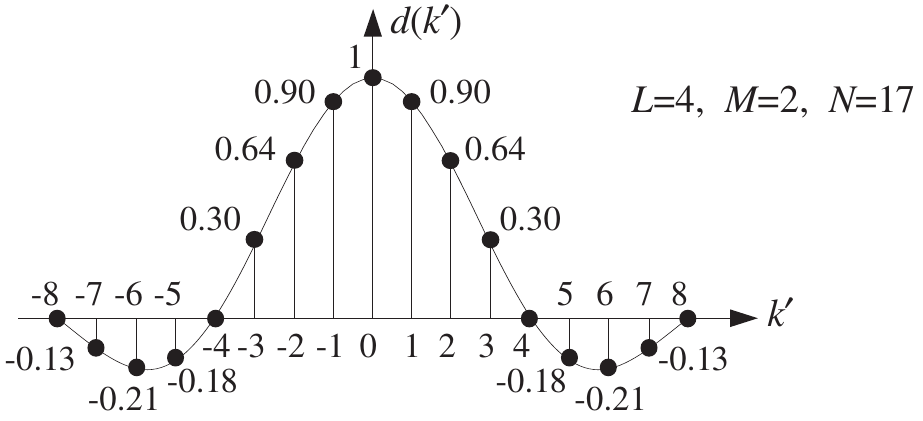
\includegraphics[width=6cm]{images/IntDecOv_DesignExample.png}
\end{center}
The interpolated samples $y_{\text{up}}(4n+i)$ between $x(n)=x_{\text{up}}(4n)$ and $x(n+1)=x_{\text{up}}(4[n+1])$ are now:
\begin{equation*}
  \begin{bmatrix}
    y_{\text{up}}(4n) \\
    y_{\text{up}}(4n+1) \\
    y_{\text{up}}(4n+2) \\
    y_{\text{up}}(4n+3)
  \end{bmatrix}
  =
  \begin{bmatrix}
        0 &    0 &    1 &     0 \\
    -0.13 & 0.30 & 0.90 & -0.18 \\
    -0.21 & 0.64 & 0.64 & -0.21 \\
    -0.18 & 0.90 & 0.30 & -0.13 \\
  \end{bmatrix}
  \begin{bmatrix}
    x_{\text{up}}(4n+8) \\
    x_{\text{up}}(4n+4) \\
    x_{\text{up}}(4n) \\
    x_{\text{up}}(4n-4)
  \end{bmatrix}
\end{equation*}
\begin{center}
  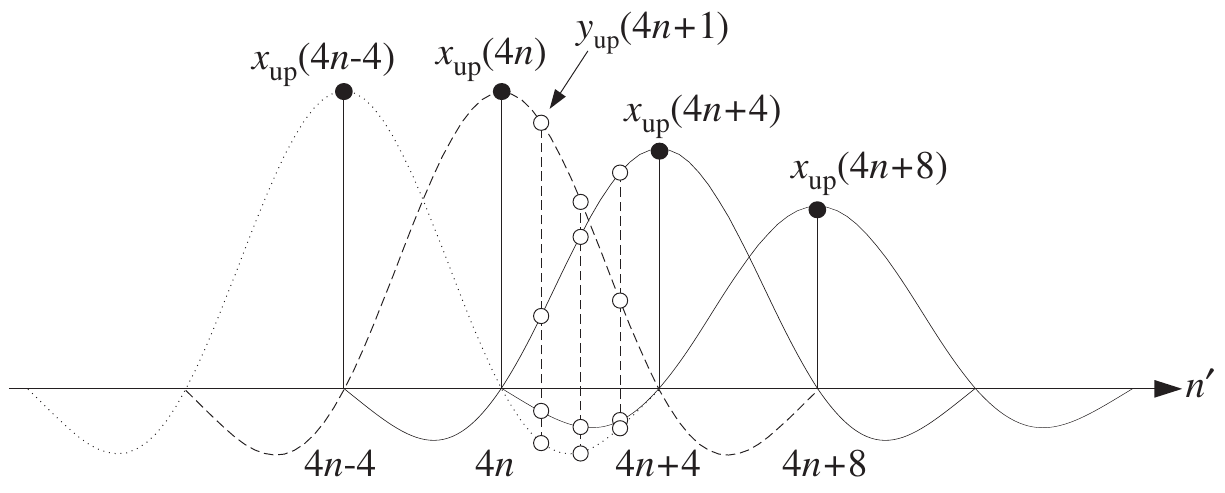
\includegraphics[width=8cm]{images/IntDecOv_DesignExampleSuperposition.png}
\end{center}

The 17 sample long FIR filter is very short ($M=2$).
This and the rectangular window have the effect that the interpolated signal is of low quality.
Rectangular windows should not be used, Hamming is much better and results in a reasonable interpolation even with $M=2$

The Hamming windowed version is obtained by multiplying the high-rate 17 sample long filter with the appropriate Hamming window resulting in
\begin{equation*}
  \begin{bmatrix}
    y_{\text{up}}(4n) \\
    y_{\text{up}}(4n+1) \\
    y_{\text{up}}(4n+2) \\
    y_{\text{up}}(4n+3)
  \end{bmatrix}
  =
  \begin{bmatrix}
        0 &    0 &    1 &     0 \\
    -0.02 & 0.22 & 0.87 & -0.07 \\
    -0.05 & 0.55 & 0.55 & -0.05 \\
    -0.07 & 0.87 & 0.22 & -0.02 \\
  \end{bmatrix}
  \begin{bmatrix}
    x_{\text{up}}(4n+8) \\
    x_{\text{up}}(4n+4) \\
    x_{\text{up}}(4n) \\
    x_{\text{up}}(4n-4)
  \end{bmatrix}
\end{equation*}
The resulting magnitude response shows, that the rectangular filter is steeper, at the high cost of 8.9\% overshoot, which the Hamming window version doesn't have.\\

For a block diagram realization of the polyphase form, recall these two relationships:
\begin{align*}
  Y_{\text{up}}(\xi) &= \sum_{i=0}^{L-1}\xi^{-1}Y_i(\xi^L) = \sum_{i=0}^{L-1}z^{-i/L}Y_i(z) \\
  D(\xi) &= \sum_{i=0}^{L-1}\xi^{-1}D_i(\xi^L) = \sum_{i=0}^{L-1}z^{-i/L}D_i(z)
\end{align*}
Therefore the transfer function of the high-rate interpolator filter can be written as the sum of the polyphase subfilters appropriately delayed:
\begin{align*}
  H(\xi) &= H_0(\xi^4) + \xi^{-1}H_1(\xi^4) + \xi^{-2}H_2(\xi^4) + \xi^{-3}H_3(\xi^4) \\
  &= H_0(z) + z^{-1/4}H_1(z) + z^{-2/4}H_2(z) + z^{-3/4}H_3(z)
\end{align*}
The resulting block diagram clearly shows how the four polyphase filters create the four output values.
Three of these values are interpolated while value $y_{\text{up}}(n') = y_{\text{up}}(4n) = y_0(n)$ is identical to the upsampled input value $x_{\text{up}}(n') = x_{\text{up}}(4n) = x(n)$, since $h_0=[0,0,1,0]$.
Clearly, the four output samples can be calculated in parallel, allowing for a very fast implementation.
\begin{center}
  \begin{tikzpicture}
    \node [inner sep=0pt,above right]
    {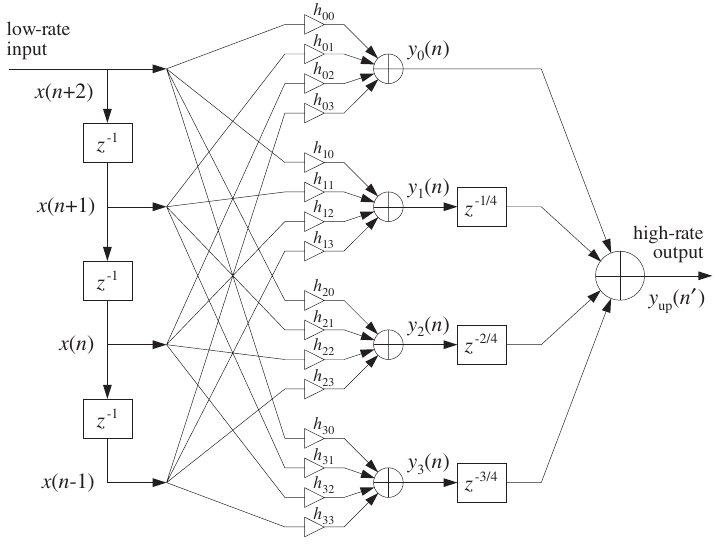
\includegraphics[width=10cm]{images/IntDecOv_DesignExamplePolyphase.png}};
    \draw[red,->] (9,7) node [right] {Missing upsampler by a factor of 4} -- (6,6.65) node {};
    \draw[red,->] (9,7) node {} -- (6,4.7) {};
    \draw[red,->] (9,7) node {} -- (6,2.75) {};
    \draw[red,->] (9,7) node {} -- (6,0.85) {};
  \end{tikzpicture}
\end{center}

\subsection{Decimation and Oversampling\buchSeite{686-691}}
Decimation is the inverse of oversampling, thus the sampling rate is reduced
from a high rate $f_s'$ to a low rate $f_s = f_s' / L$.

\begin{center}
	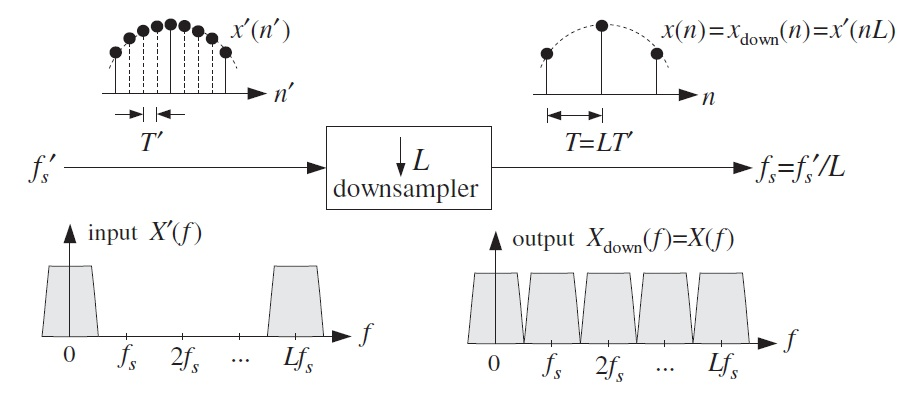
\includegraphics[width=10cm]{images/IntDecOv_Downsampler.jpg}
\end{center}

Downsampling is simply the process of discarding $L-1$ samples:

\begin{equation*}
	x_{down}(n) = \left.x'(n')\right|_{n'=nL} = x'(nL)
\end{equation*}

Caution: if the high rate spectrum occupies more than the low rate Nyquist rate
there \emph{will} be aliasing. \\

The ideal \emph{decimator} therefore contains a decimation filter, which
operates at the high frequencies and cuts out the low rate Nyquist band.

\begin{center}
	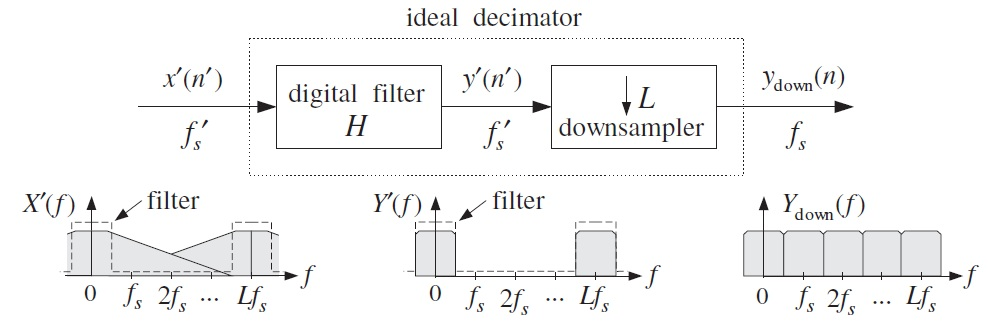
\includegraphics[width=12cm]{images/IntDecOv_Decimator.jpg}
\end{center}

The decimation filter is similar to the interpolation filter, except that
its DC gain is unity instead of $L$. A length-$N$ FIR decimation filter
can therefore be obtained by

\begin{equation*}
	h(n') = w(n') d(n'-LM) \:,\qquad \text{where} \quad
	d(k') = \frac{\sin(\pi k'/L)}{\pi k'}
\end{equation*}

Since only every $L$th output sample is needed, the filter output does
not need to be calculated for every fast rate sample (like on the left image),
reducing the computational cost by a factor $L$ to
$R = \frac{1}{L} N f_s' = N f_s$ (left image). \\

\begin{multicols}{2}
	\begin{center}
		\adjustbox{max width=0.9\linewidth}{\begin{tikzpicture}
[	
	sq/.style={rectangle,draw,line width=1,minimum height=1cm,minimum width=1cm}
]

\node[sq] (t1) at (1,0) {$\zeta^{-1}$};
\node[sq] (t2) at (3,0) {$\zeta^{-1}$};
\node[sq] (t3) at (5,0) {$\zeta^{-1}$};

\node[sq] (c1) at (0,-2) {$C_0$};
\node[sq] (c2) at (2,-2) {$C_1$};
\node[sq] (c3) at (4,-2) {$C_2$};
\node[sq] (c4) at (6,-2) {$C_3$};

\node[rectangle,draw,line width=1,minimum height=1cm, minimum width=8cm] (sum) at (3,-4) {$\sum$};
\node[sq] (ds) at (9,-4) {$\downarrow 4$};

\draw[thick,->]	(-1,0)	-- 	(t1);
\draw[thick,->]	(t1)		-- 	(t2);
\draw[thick,->]	(t2) 		-- 	(t3);

\draw[thick,->] (-1,0)	-|	(c1);
\draw[thick,->] (t1)		-|	(c2);
\draw[thick,->] (t2)		-|	(c3);
\draw[thick,->] (t3)		-|	(c4);

\draw[thick,->] (c1) 		-- 	(0,-3.5);
\draw[thick,->] (c2) 		-- 	(2,-3.5);
\draw[thick,->] (c3) 		-- 	(4,-3.5);
\draw[thick,->] (c4) 		-- 	(6,-3.5);

\draw[thick,->] (sum) -- (ds);
\draw[thick,->] (ds) -- (10,-4);

\end{tikzpicture}} \\
	\end{center}
\vfill\columnbreak
	\begin{center}
		\adjustbox{max width=0.7\linewidth}{\begin{tikzpicture}
[	
	sq/.style={rectangle,draw,line width=1,minimum height=1cm,minimum width=1cm}
]

\node[sq] (t1) at (1,0) {$\zeta^{-1}$};
\node[sq] (t2) at (3,0) {$\zeta^{-1}$};
\node[sq] (t3) at (5,0) {$\zeta^{-1}$};

\node[sq] (d1) at (0,-1.5) {$\downarrow 4$};
\node[sq] (d2) at (2,-1.5) {$\downarrow 4$};
\node[sq] (d3) at (4,-1.5) {$\downarrow 4$};
\node[sq] (d4) at (6,-1.5) {$\downarrow 4$};

\node[sq] (c1) at (0,-3) {$C_0$};
\node[sq] (c2) at (2,-3) {$C_1$};
\node[sq] (c3) at (4,-3) {$C_2$};
\node[sq] (c4) at (6,-3) {$C_3$};

\node[rectangle,draw,line width=1,minimum height=1cm, minimum width=8cm] (sum) at (3,-4.5) {$\sum$};


\draw[thick,->]	(-1,0)	-- 	(t1);
\draw[thick,->]	(t1)		-- 	(t2);
\draw[thick,->]	(t2) 		-- 	(t3);

\draw[thick,->] (-1,0)	-|	(d1);
\draw[thick,->] (t1)		-|	(d2);
\draw[thick,->] (t2)		-|	(d3);
\draw[thick,->] (t3)		-|	(d4);

\draw[thick,->]	(d1)		-- 	(c1);
\draw[thick,->]	(d2)		-- 	(c2);
\draw[thick,->]	(d3)		-- 	(c3);
\draw[thick,->]	(d4)		-- 	(c4);

\draw[thick,->] (c1) 		-- 	(0,-4);
\draw[thick,->] (c2) 		-- 	(2,-4);
\draw[thick,->] (c3) 		-- 	(4,-4);
\draw[thick,->] (c4) 		-- 	(6,-4);

\draw[thick,->] (sum) -- (8,-4.5);

\end{tikzpicture}} \\
	\end{center}
\end{multicols}

Multistage designs are very popular for decimation filters. The early filters will
then be fast but simple, while later filters are slow but very precise. For fast
signals, often a simple FIR averaging filter is used. The last, slowest filter
can then be designed to fix the overall frequency response.


\subsection{Noise Shaping Quantizer\buchSeite{698-705}}

\paragraph{First-order delta-sigma A/D converters}
For first order delta-sigma A/D converters, only one bit is used: $B'=1$. For
slow signals, the quantization error will be small. The system will therefore
be oversampled such that the quantization noise is moved into higher frequencies,
which are then suppressed by the digital decimation filter.

\begin{center}
	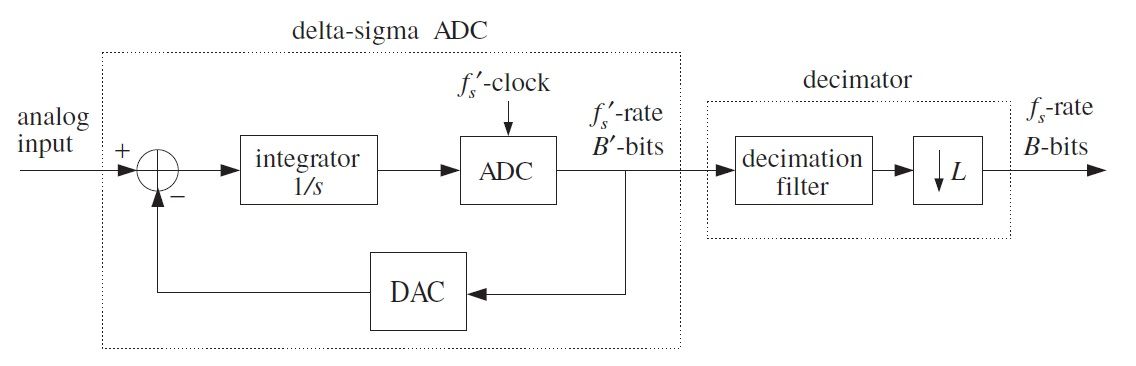
\includegraphics[width=11cm]{images/IntDecOv_SigmaDelta.jpg}
\end{center}

To be able to create a discrete time model, we replace the quantizer by
an additive quantization noise model.

\begin{center}
	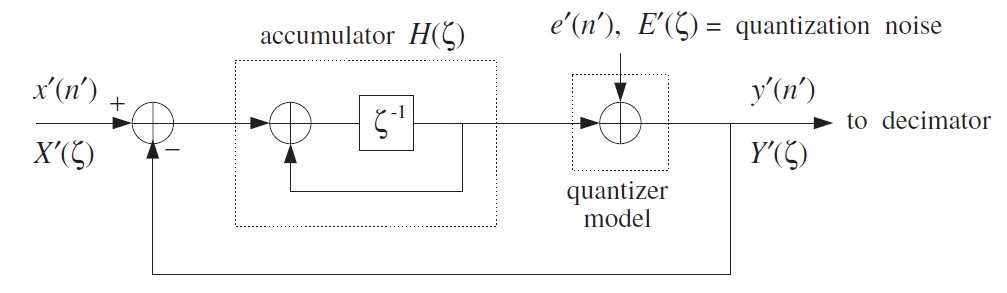
\includegraphics[width=10cm]{images/IntDecOv_SigmaDeltaModel.jpg}
\end{center}

The transfer functions for the input $X$ and the noise $NS$ will then be

\begin{equation*}
	H_X(\zeta) = \zeta^{-1} \qquad H_{NS}(\zeta) = 1 - \zeta^{-1}
\end{equation*}

or for higher orders $p$: $H_{NS}(\zeta) = (1-\zeta^{-1})^p$. \\

The MSE is obtained by
\begin{equation*}
  \sigma_e^2 = \sigma_{e'}^2 \frac{1}{f_s^{'}} \int_{-f_s/2}^{f_s/2} |H_{NS}(f)|^2 df
\end{equation*}
with $f_s^{'} = L f_s$ and
\begin{equation*}
  |H_{NS}(f)|^2 = |2 \sin(\frac{\pi f}{f_s^{'}})|^{2p}
\end{equation*}

This leads to the known relationship of

\begin{equation*}
	\Delta B = (p+0.5) \log_2 L - 0.5 \log_2\left(\frac{\pi^{2p}}{2p+1}\right)
\end{equation*}


\paragraph{Oversampled noise shaping requantizers for D/A conversion}
Similarly, noise shaping and oversampling can be used for D/A conversion.

\begin{center}
	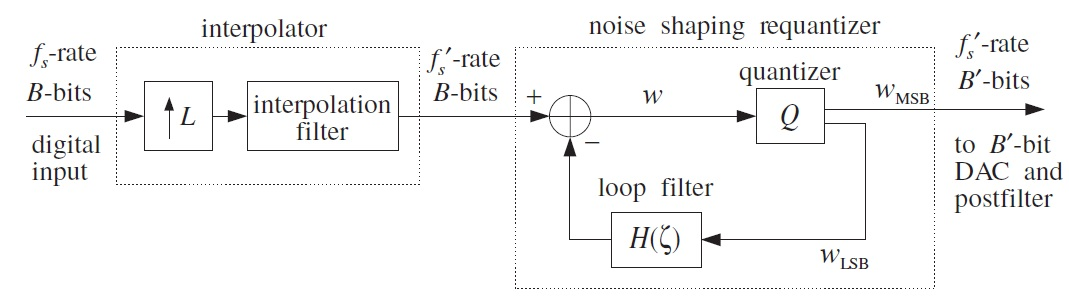
\includegraphics[width=12cm]{images/IntDecOv_Requantizer.jpg}
\end{center}

Again, using a discrete time model and a linear stochastic quantization
noise source, one gets to the following transfer functions for first-order
or higher-order noise shaping filters

\begin{align*}
	H(\zeta) &= \zeta^{-1} \qquad &
	H_{NS}(\zeta) &= (1-\zeta^{-1}) \qquad
	& \text{first-order} \\
	H(\zeta) &= 2 \zeta^{-1} - \zeta^{-2} \qquad &
	H_{NS}(\zeta) &= (1-\zeta^{-1})^2 \qquad
	& \text{second-order}
\end{align*}

and again

\begin{equation*}
	\Delta B = (p+0.5) \log_2 L - 0.5 \log_2\left(\frac{\pi^{2p}}{2p+1}\right)
\end{equation*}


% Idiotenseite
\appendix
\section{Idiotenseite}
\addtocontents{toc}{\protect\setcounter{tocdepth}{-1}}
\input{idiotenseite/trigo/subsections/Winkelargumente}
\input{idiotenseite/trigo/subsections/Quadrantenbeziehungen}
\input{idiotenseite/trigo/subsections/Periodizitaet}
\begin{multicols}{2}
\input{idiotenseite/trigo/subsections/Additionstheoreme}
\input{idiotenseite/trigo/subsections/DoppelHalbwinkel}
\input{idiotenseite/trigo/subsections/Produkte}
\input{idiotenseite/trigo/subsections/SummeDifferenzen}
\input{idiotenseite/trigo/subsections/Euler}

\end{multicols}
\input{idiotenseite/diverses/subsections/Reihenentwicklung}

\end{document}

